\documentclass[dvipsnames,10pt]{beamer}
\usepackage{ucltemplate}
\usepackage{tikz}
\usetikzlibrary{arrows,shapes, backgrounds, decorations.pathmorphing}
\usepackage{graphicx}
\usepackage{amssymb,amsmath}
\usepackage{listings}
\usepackage{dcolumn}
\usepackage{multirow}
\usepackage{multimedia}
\usepackage{empheq}
\usepackage{makecell}
\usepackage[many]{tcolorbox}
\usepackage[labelformat=empty]{caption,subfig}
\usepackage[export]{adjustbox}

%\usepackage[usenames]{color}
%\usetheme{Madrid}
%\mode<presentation>
\setbeamertemplate{navigation symbols}{}
\tikzstyle{na} = [baseline=-.5ex]

\tcbset{highlight math style={enhanced,
  colframe=red!60!black,colback=yellow!50!white,arc=4pt,boxrule=1pt,
  }}

\def\bx{\mathbf{x}}
\def\by{\mathbf{y}}

\renewcommand\theadalign{bc}
\renewcommand\theadfont{\bfseries}
\renewcommand\theadgape{\Gape[4pt]}
\renewcommand\cellgape{\Gape[4pt]}

% From https://tex.stackexchange.com/questions/60216/how-to-create-a-squiggle-arrow-with-some-text-on-it-in-tikz
\newcounter{sarrow}
\newcommand\xrsquigarrow[1]{%
\stepcounter{sarrow}%
\begin{tikzpicture}[decoration=snake]
\node (\thesarrow) {\strut#1};
\draw[->,decorate] (\thesarrow.south west) -- (\thesarrow.south east);
\end{tikzpicture}%
}

\title{A rusty roadmap to integral equations at exascale}
%\author{\texorpdfstring{Timo Betcke\newline\url{t.betcke@ucl.ac.uk}}{Betcke}}

%\institute[University College London]{Department of Mathematics \\
%  University College London}
\date{}

\begin{document}
\lstset{language=Python}
\tikzstyle{every picture}+=[remember picture]
\begin{frame}
% \vspace*{-0.94cm}
% \hspace*{-1.02cm}
%\noindent\includegraphics[scale=0.4]{1824logo}

% \vspace{-3cm}
\vspace{1cm}

\titlepage
\vspace{-2cm}
\begin{columns}[T]
\begin{column}{.48\textwidth}
\begin{center}
    Timo Betcke \\
    \url{t.betcke@ucl.ac.uk}\\
    University College London
\end{center}
\begin{tcolorbox}
Joint with S. Kailasa, M. Scroggs and many
other collaborators
\end{tcolorbox}
\end{column}%
\hfill%
\begin{column}{.48\textwidth}
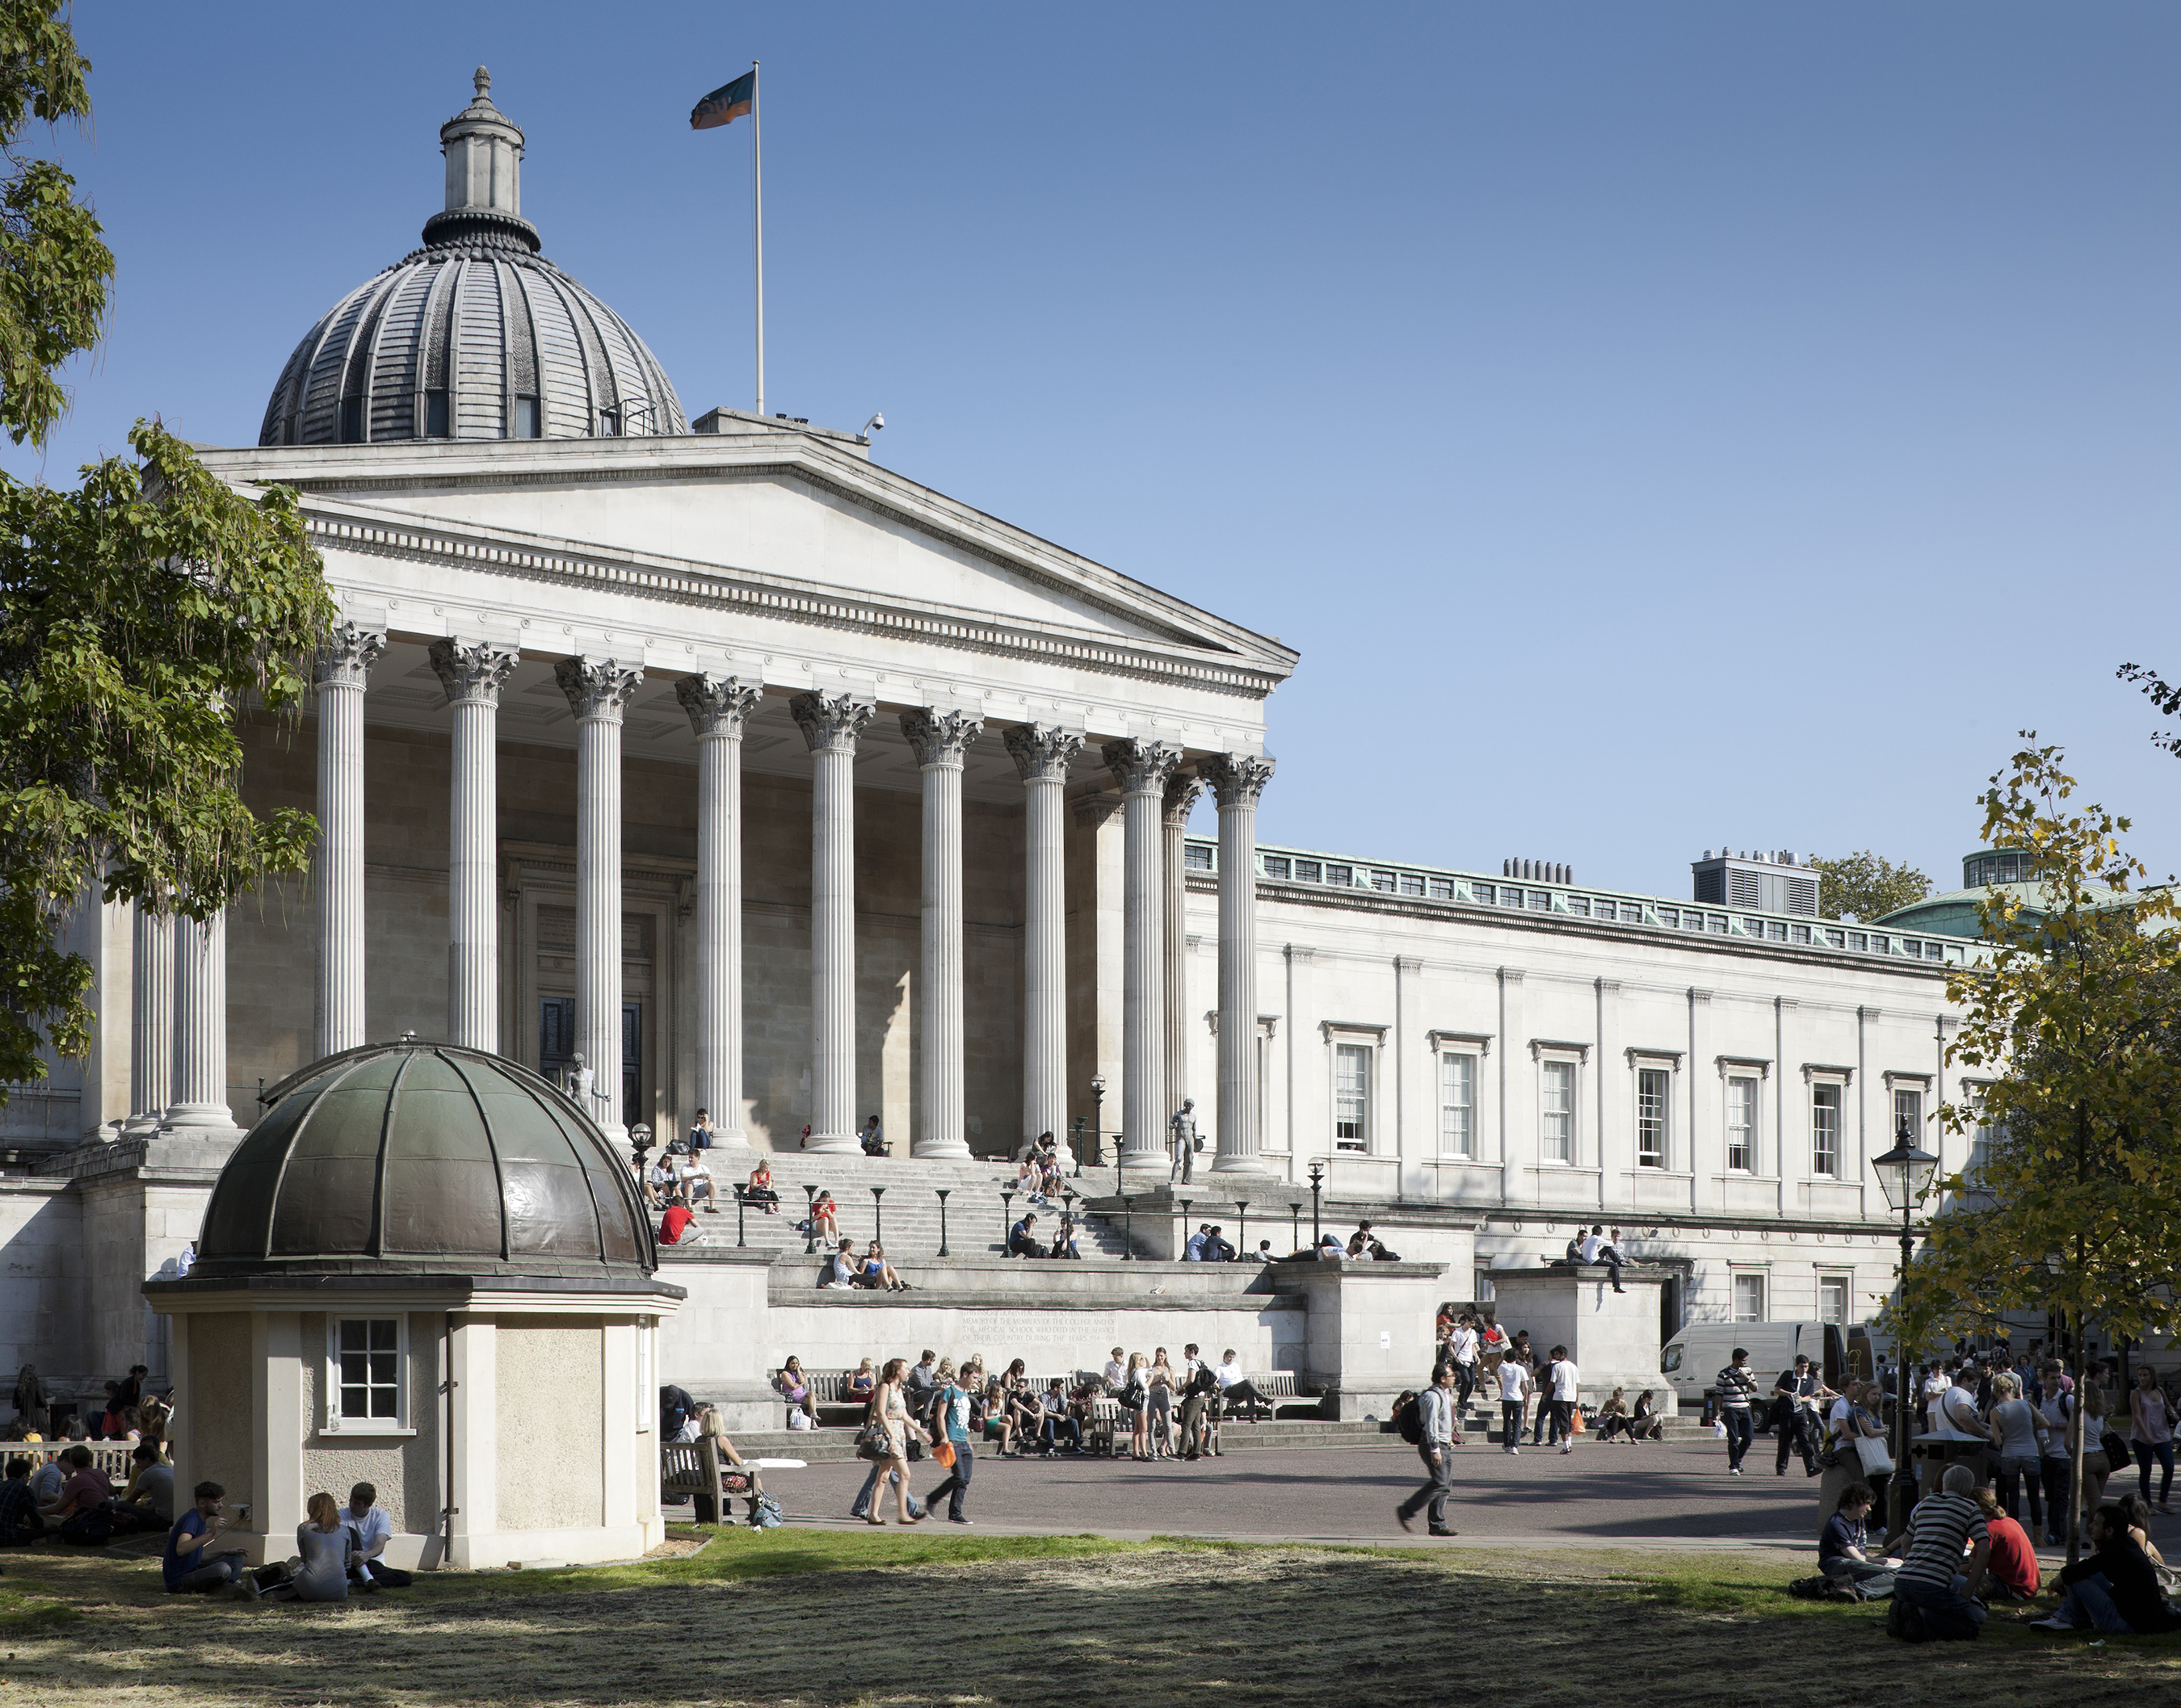
\includegraphics[width=5cm]{../figs/ucl_campus}

\end{column}%
\end{columns}

\end{frame}

\begin{frame}
	\frametitle{Some Maths to set the stage}
	
    \begin{minipage}{5cm}
    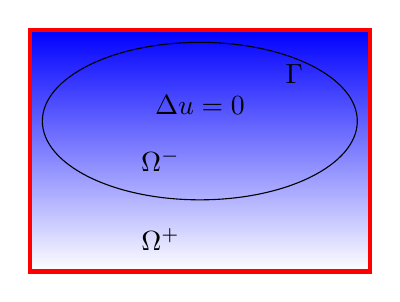
\begin{tikzpicture}[scale=1, framed,background rectangle/.style={ultra thick,draw=red, top color=blue}]
        \draw (0,0) ellipse (2cm and 1cm);
        \draw (.0,.2) node {$\Delta u = 0$};
        \draw (-.5, -.5) node {$\Omega^{-}$};
        \draw (1.2, .6) node {$\Gamma$};
        \draw (-.5, -1.5) node {$\Omega^{+}$};
    \end{tikzpicture}
\end{minipage}
\begin{minipage}{5cm}
$$
\Delta u(\bx) := \frac{\partial^2 u}{\partial x^2} + \frac{\partial^2 u}{\partial y^2} + \frac{\partial^2 u}{\partial z^2}
$$
Application areas: Heat diffusion, electrostatics, etc.

\vspace{\baselineskip}
Boundary condition:\\ $u(\bx) = f(\bx)$.


\end{minipage}

\vspace{.5cm}

Represent solution as

	\begin{tcolorbox}
	$$
	u(\bx) = \int_{\Gamma} g(\bx, \by)\phi(\by)ds(\by),\quad \bx\in\Omega 
	$$
	\end{tcolorbox}

	Need to solve $V\phi = f$ with
	$$
	[V\phi](\bx) = \int_{\Gamma} g(\bx, \by)\phi(\by)ds(\by),\quad \bx\in\Gamma
	$$

	

	
\end{frame}
	
\begin{frame}{How to discretise the integral equation?}
We want to solve $V\phi = f$. Introduce a triangulation $\mathcal{T}$ of the domain $\Omega$ into triangles $\tau_j$. Define basis fct.
$$
\phi_j(\bx) = \left\{\begin{array}{cc} 1 & \bx \in \tau_j\\ 0, & \text{ otherwise }\end{array}\right.
$$
We approximate $\phi = \sum_{j=1}^Nc_j\phi_j$. Multiplying with $\phi_i$ and integrating gives
$$
\int_{\Gamma}\phi_i(\bx)\left[V\phi\right](\bx)ds(\bx) = \int_{\Gamma}f(\bx)\phi_i(\bx)ds(\bx), i=1, \dots, N
$$
\begin{columns}[T]
\begin{column}{0.48\textwidth}
Solve $\mathbf{V}\mathbf{c} = \mathbf{b}$
\begin{align}
\mathbf{V}_{ij} &= \int_{\tau_i}\int_{\tau_j} g(\bx, \by)ds(\by) ds(\bx)\nonumber\\
\mathbf{b}_i &= \int_{\Gamma}f(\bx)\phi_i(\bx)ds(\bx)\nonumber
\end{align}
\end{column}
 \begin{column}{0.48\textwidth}
\vspace{-.5cm}
 \begin{center}
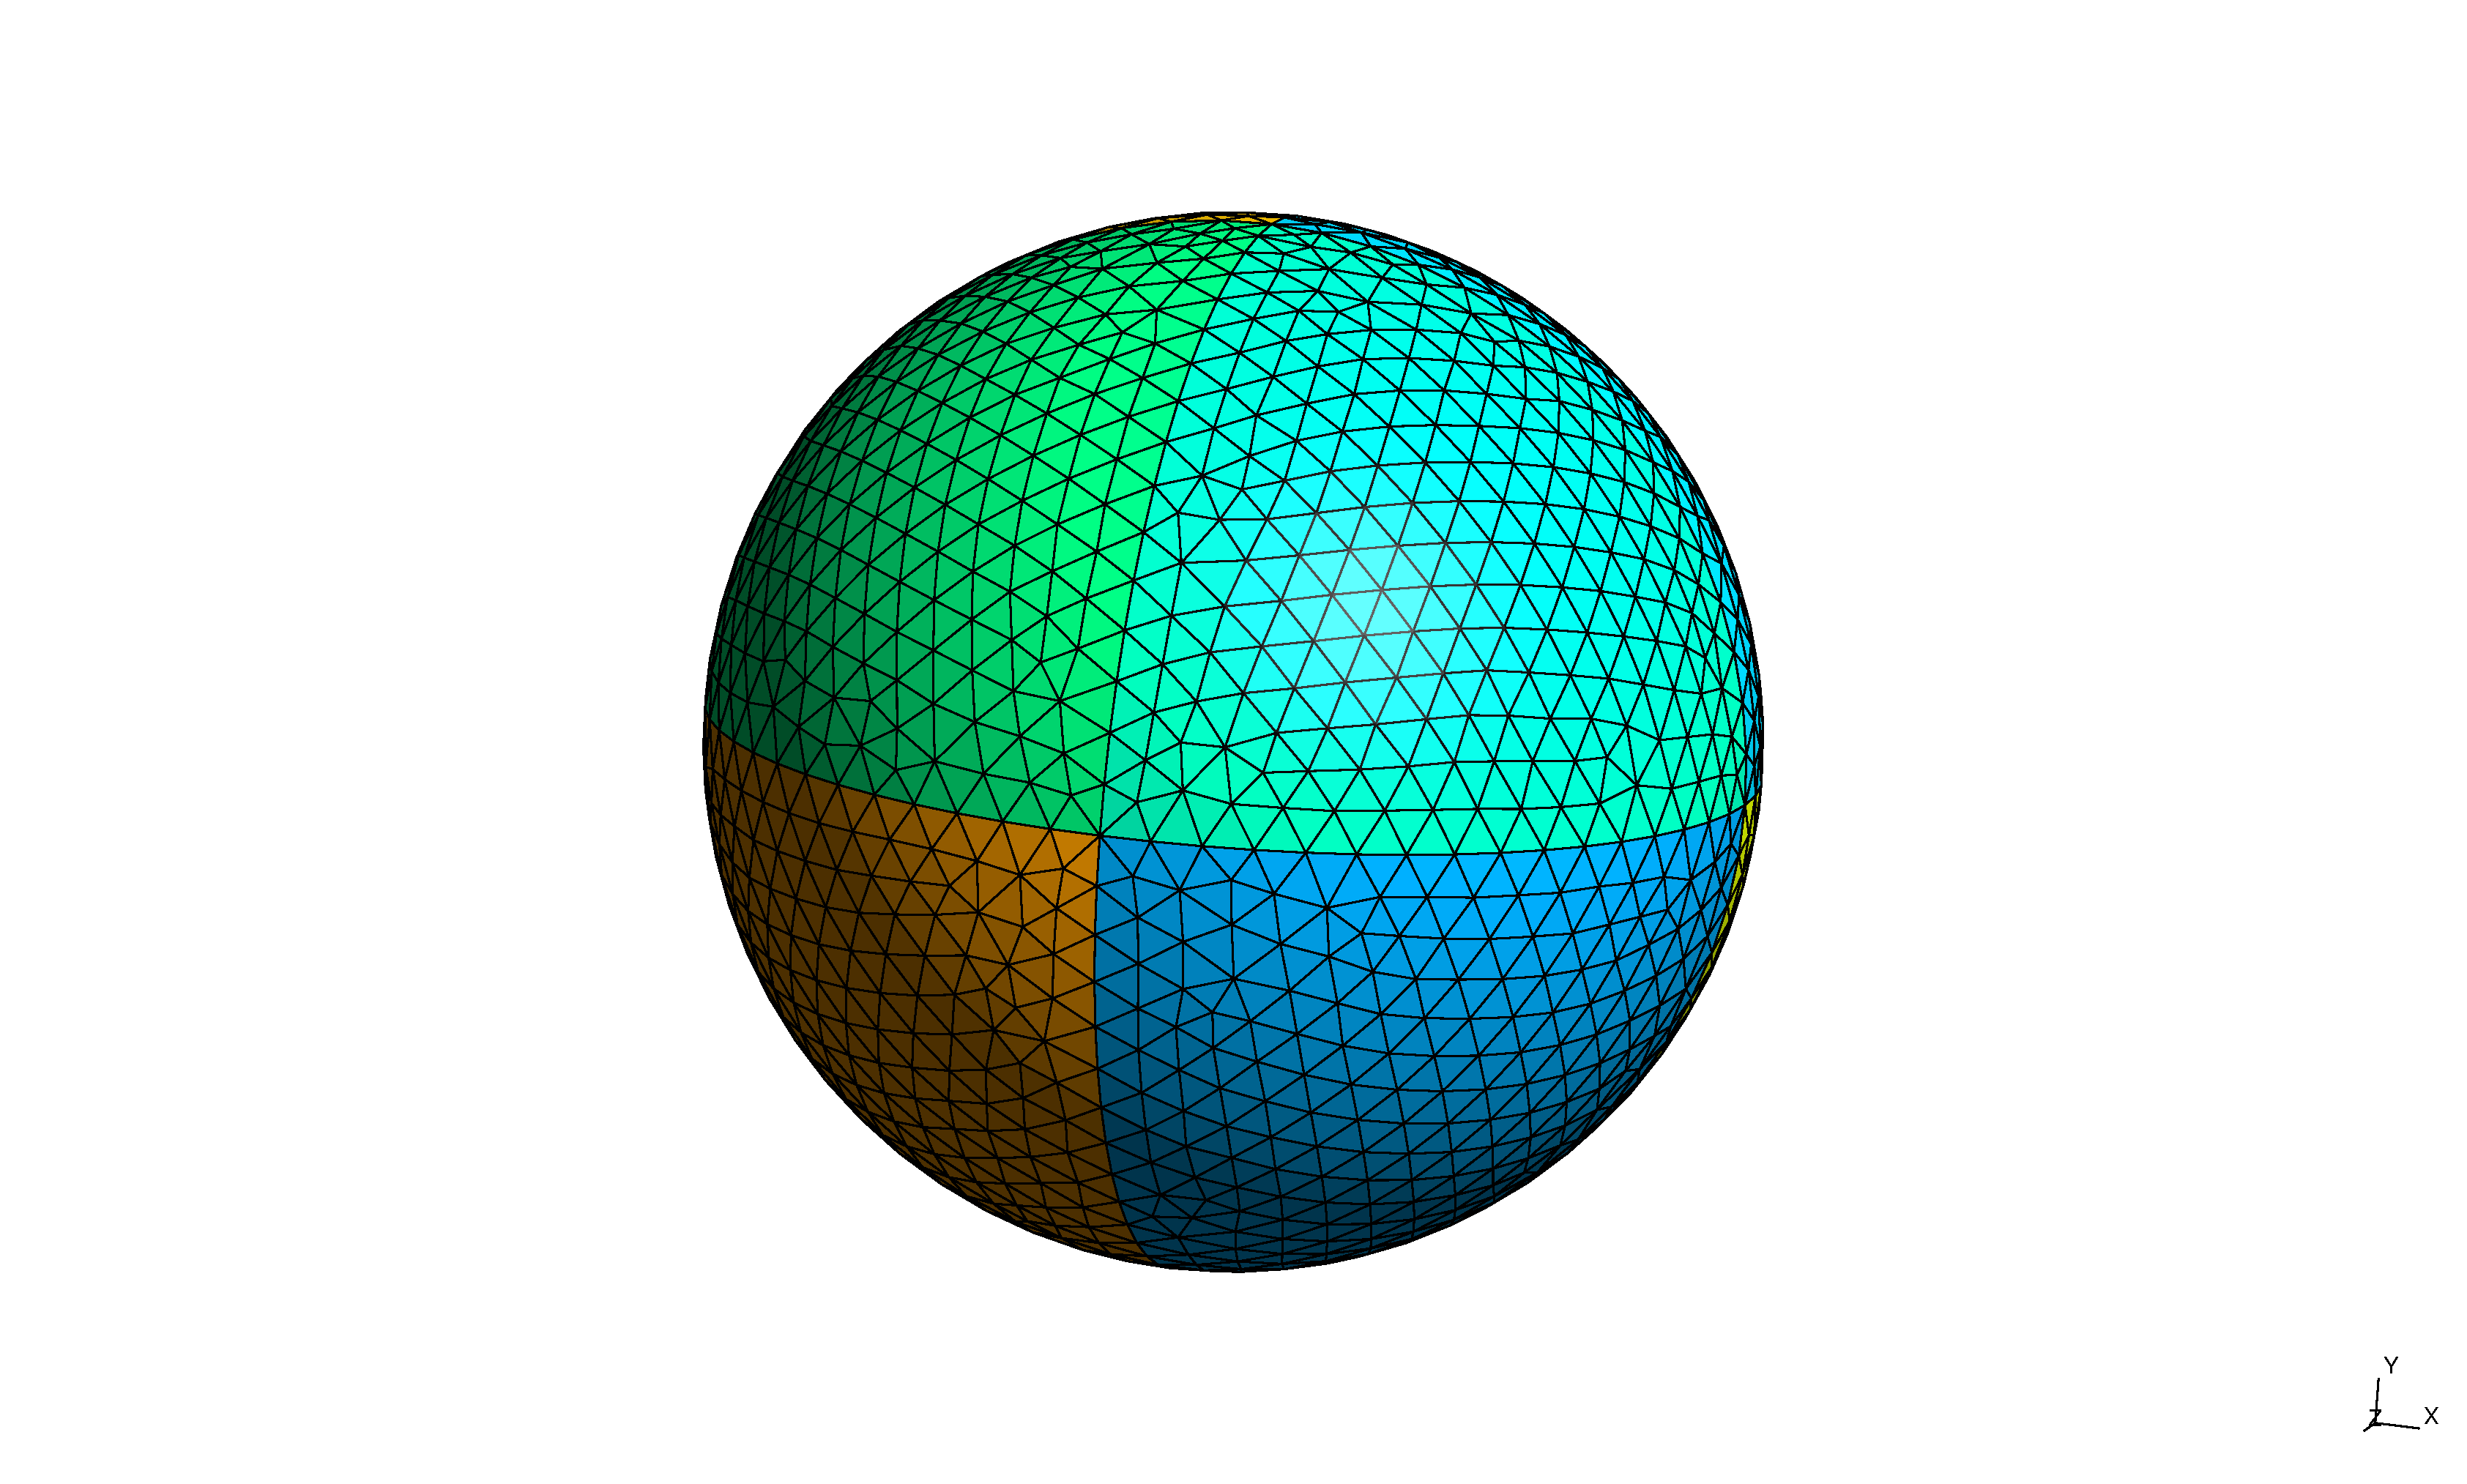
\includegraphics[width=5cm]{../figs/sphere.pdf}
\end{center}
 \end{column}
 \end{columns}  
\end{frame}


	
\begin{frame} 
	\frametitle{The Bempp boundary element software}

\begin{center}
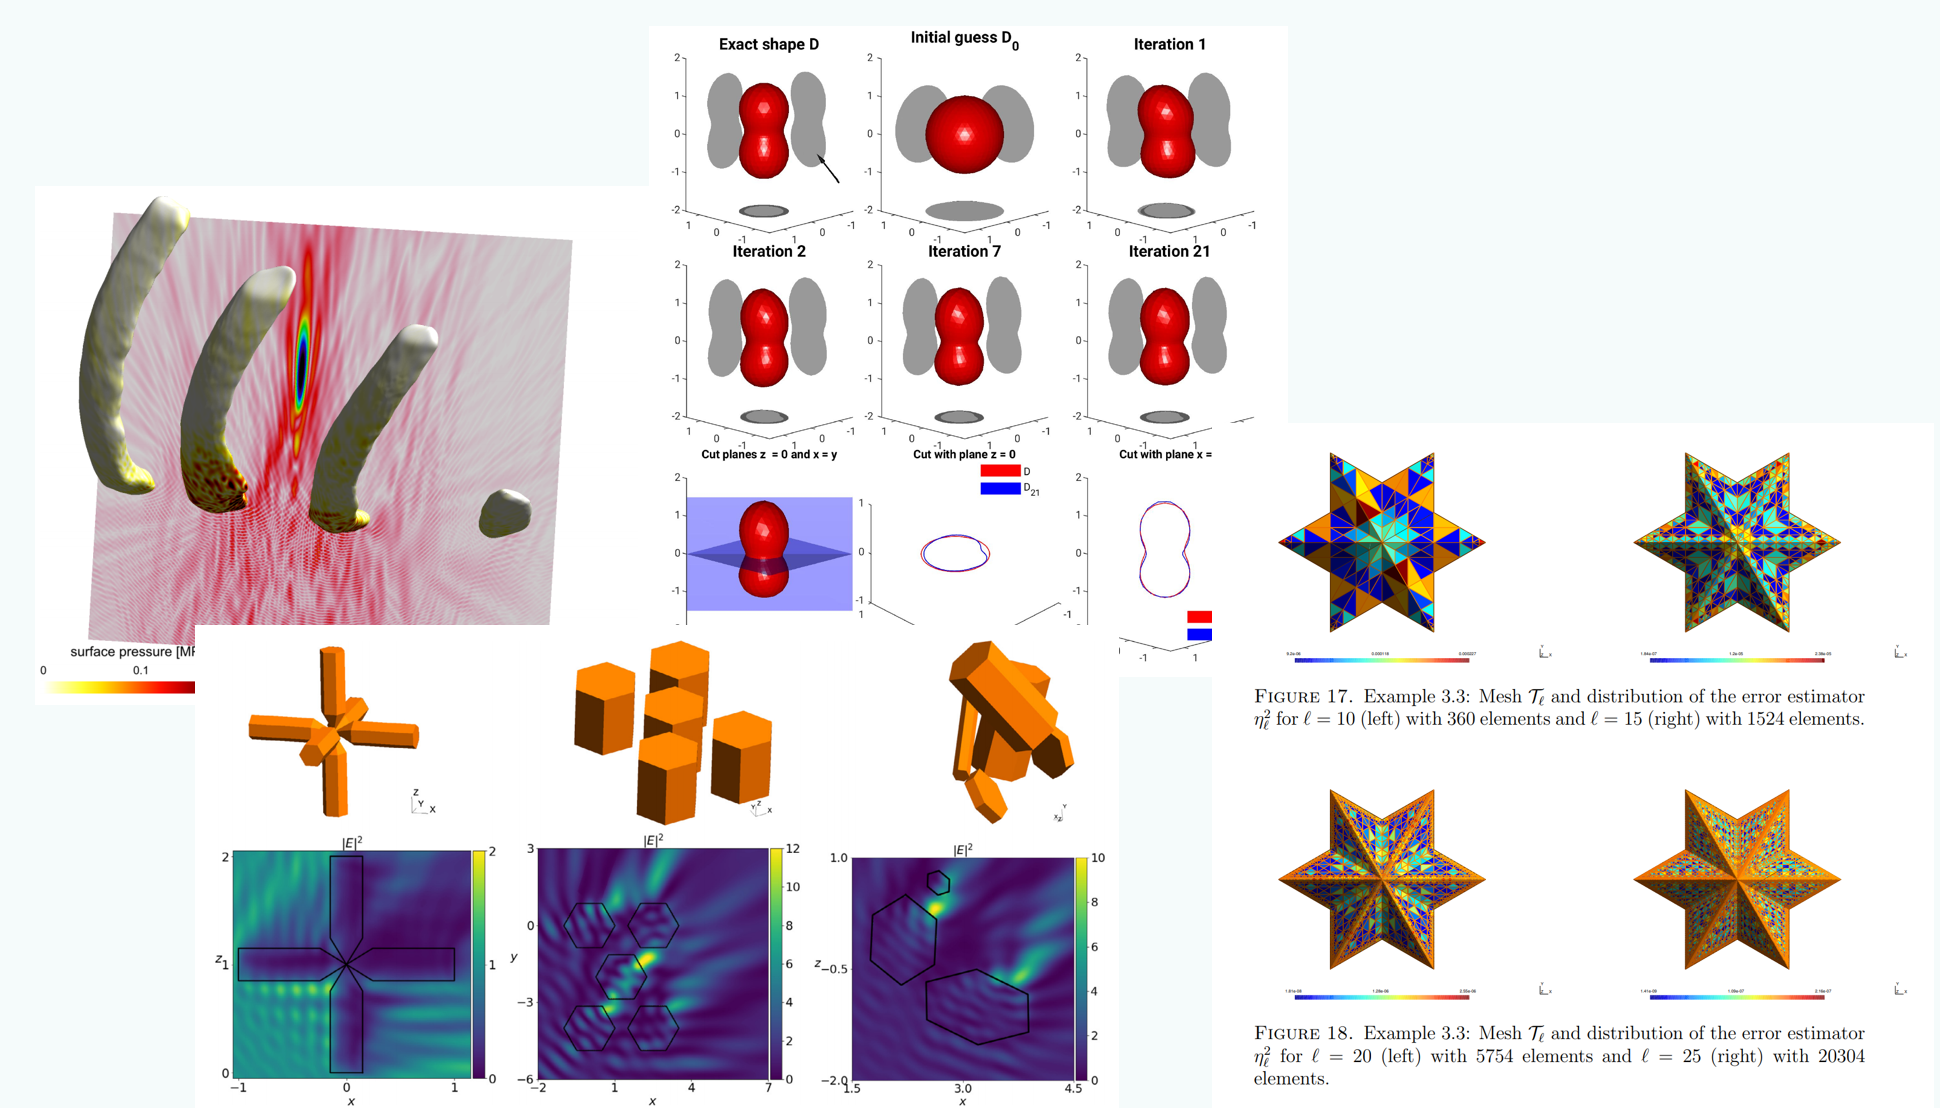
\includegraphics[width=11cm]{../figs/applications}
\end{center}

\end{frame}


\begin{frame}{Fast JIT compiled Galerkin BEM in Python}

\begin{minipage}{5cm}
\begin{small}
{\color{blue} Numba for grid iterations}
\begin{itemize}
    \item Grid topology computations
    \item Python callables
    \item Routines on grid functions, ($L^2$-norm, etc.)
    \item Fallback for operators
\end{itemize}
\end{small}
\end{minipage}
\begin{minipage}{5cm}
\vspace{-.6cm}
\begin{small}
{\color{blue} OpenCL for matrix assembly/evaluation}
\begin{itemize}
    \item All potential evaluations
    \item Mass matrices
    \item FMM Near-Field
\end{itemize}
\end{small}
\end{minipage}

\vspace{\baselineskip}

\begin{small}
{\color{blue} Other technologies }
\begin{itemize}
    \item Scipy for spare matrix operations and iterative solvers
    \item Numpy dense solvers
\end{itemize}
\end{small}

\vspace{\baselineskip}

\begin{tcolorbox}
\begin{itemize}
\item All logic controlled from Python (easy to hack on).
\item Very fast SIMD optimized dense matrix assembly.
\item But need lots of OpenCL C99 kernel code.
\end{itemize}
\end{tcolorbox}

\end{frame}

\begin{frame}
    \frametitle{Characteristics of Bempp-cl\footnote{\tiny T. Betcke, M. Scroggs, \textit{Designing a high-performance boundary element library with OpenCL and Numba}, Computing in Science and Engineering, 23 (2021), pp. 18 - 28}}
    \vspace{-.1cm}
    \begin{center}
        \begin{tabular}{cc}
            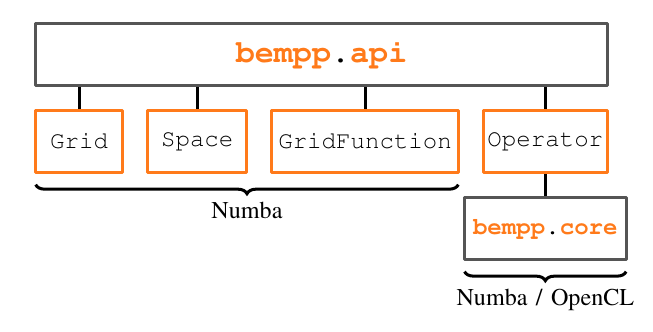
\includegraphics[width=4cm]{../figs/bempp_cl_overview.png} & 
            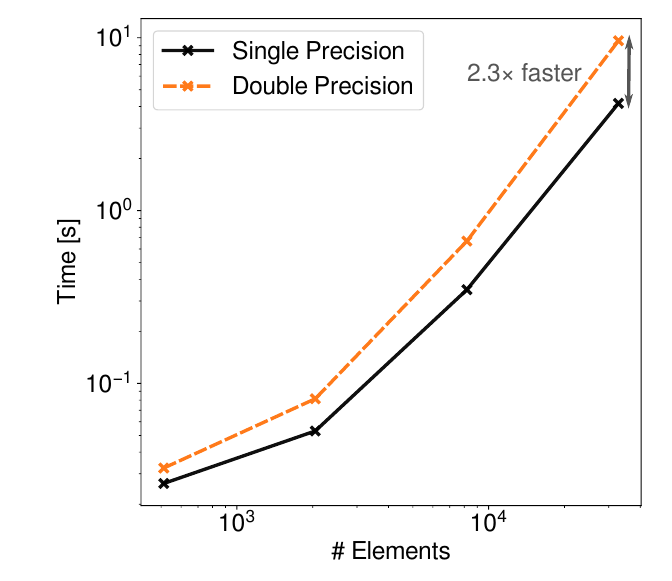
\includegraphics[width=4cm]{../figs/bempp_single_vs_double.png} \\
            \begin{minipage}{5cm}
                \vspace{-3cm}
                \begin{itemize}
                    \item Top: Structure of Bempp-cl
                    \item Top-Right: AVX acceleration in Bempp-cl
                    \item Bottom-Right: Offloading of a domain potential operator
                \end{itemize}
            \end{minipage}&
            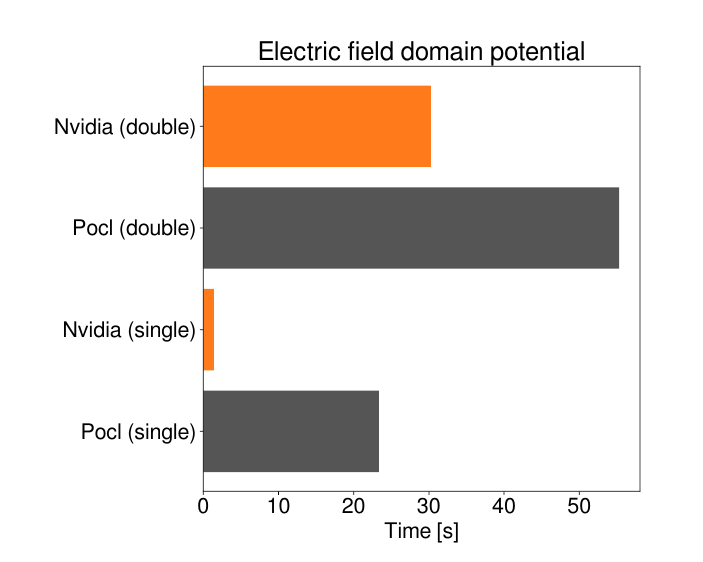
\includegraphics[width=4cm]{../figs/gpu_offloading.png} 
        \end{tabular}
    \end{center}
\end{frame}

\begin{frame}
    \frametitle{Exafmm-t: High-Performance KIFMM\footnote{\tiny T. Wang, R. Yokota, L. Barba, \textit{ExaFMM: a high-performance fast multipole method library with C++ and Python interfaces}, Journal of Open Source Software 6(61), 3145}}
    \vspace{-.1cm}
    \begin{center}
        \begin{tabular}{cc}
            \begin{minipage}{5cm}
                \begin{itemize}
                    \item Kernel-Independent FMM library.
                    \item Written in C++, Provides Python Interface.
                    \item Highly efficient at higher accuracies.
                \end{itemize}
            \end{minipage} &
            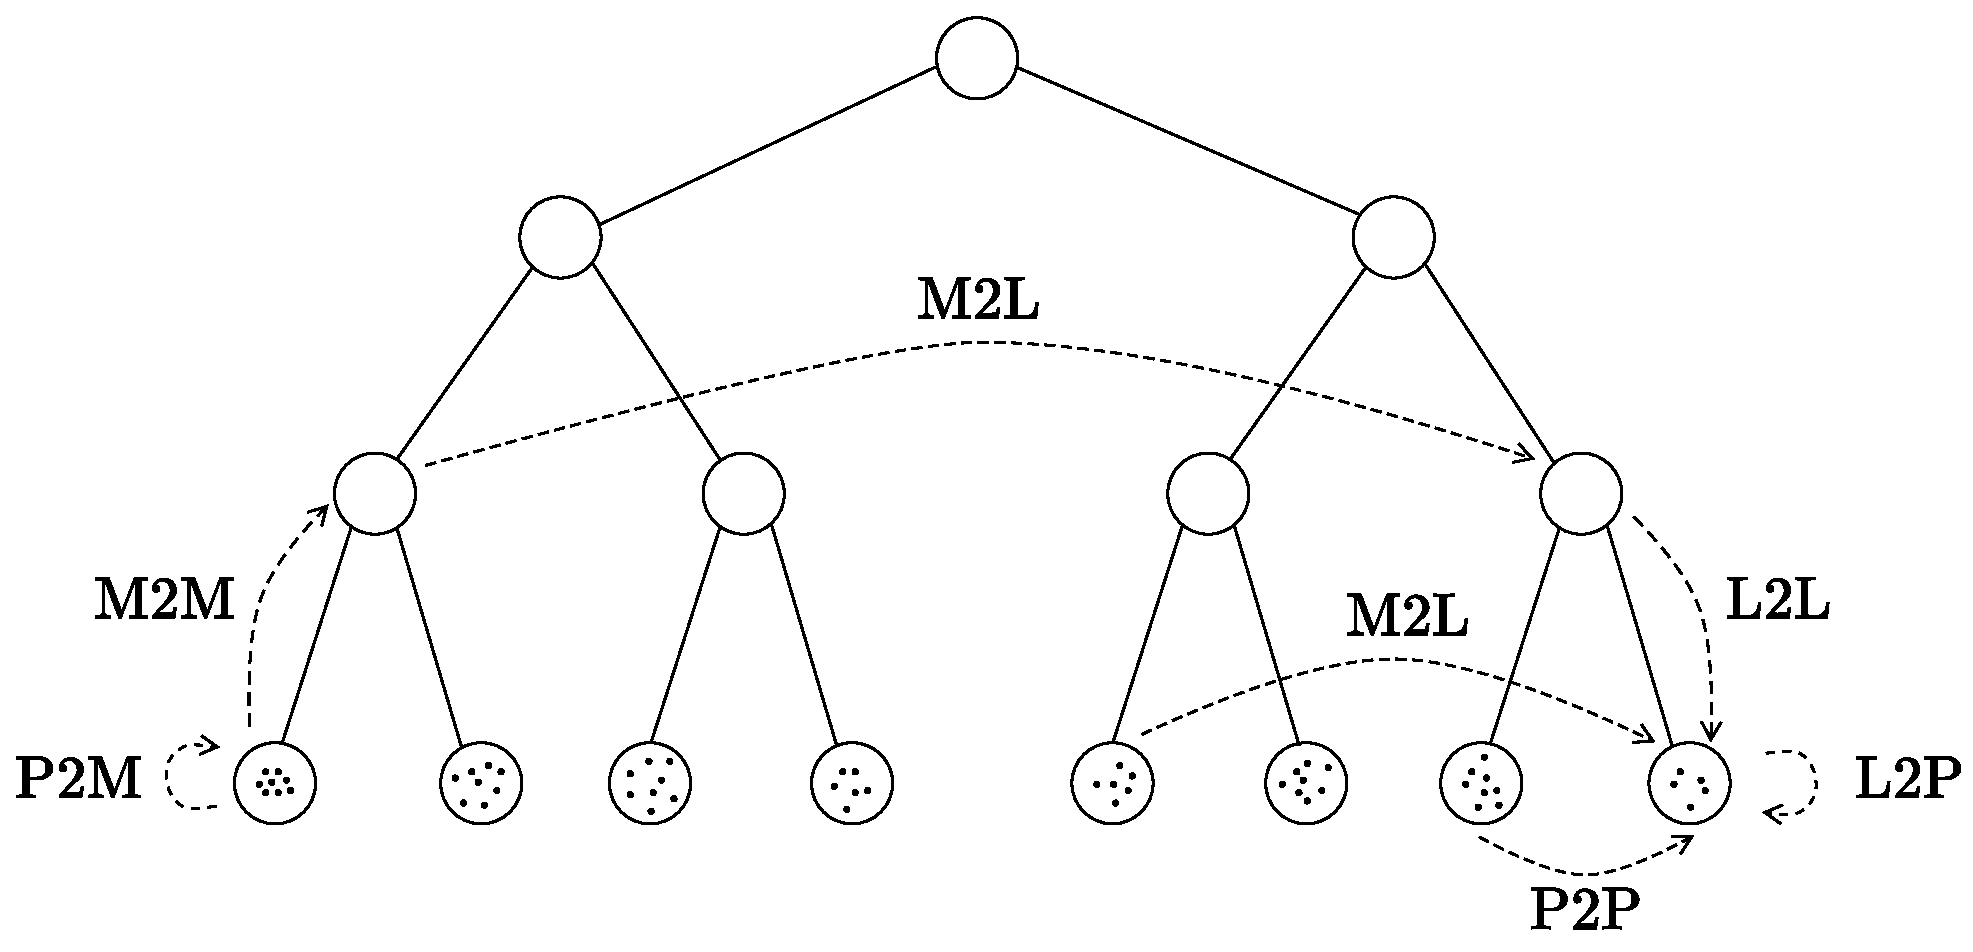
\includegraphics[width=5cm]{../figs/fmm_sketch.pdf} \\
            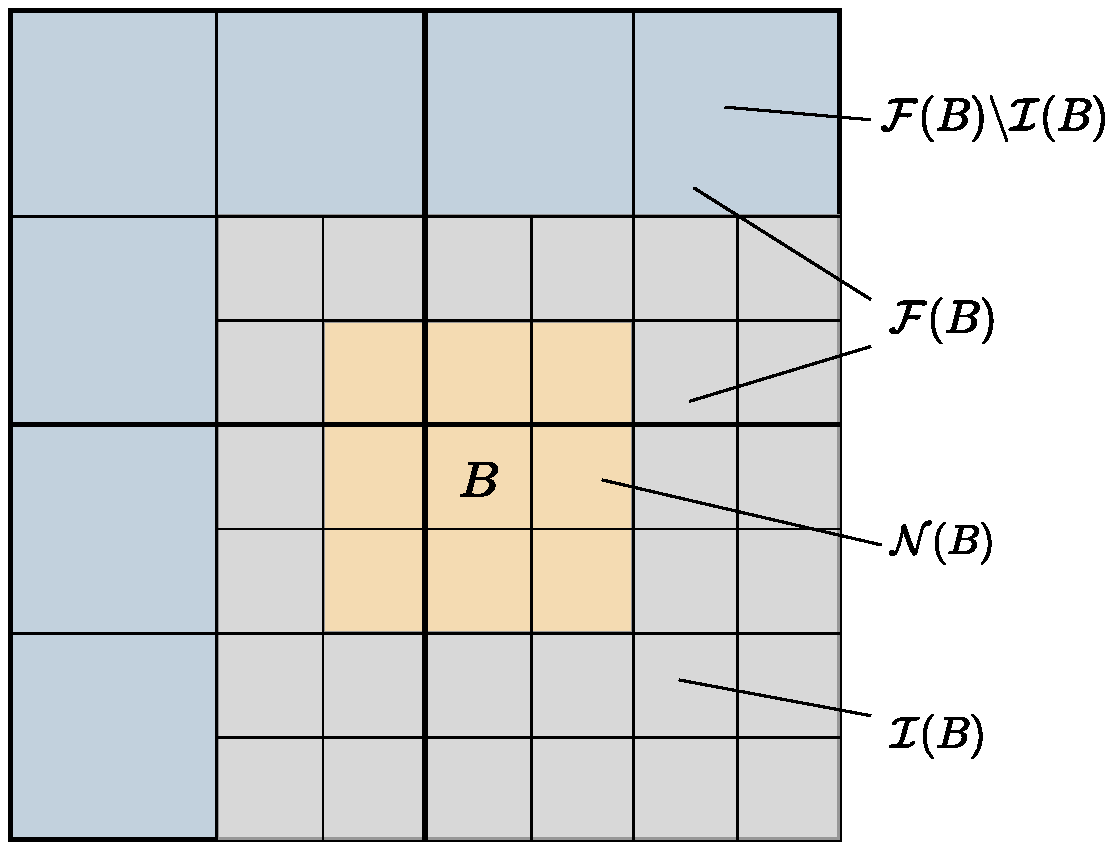
\includegraphics[width=4cm]{../figs/near_far_decomposition.pdf} &
            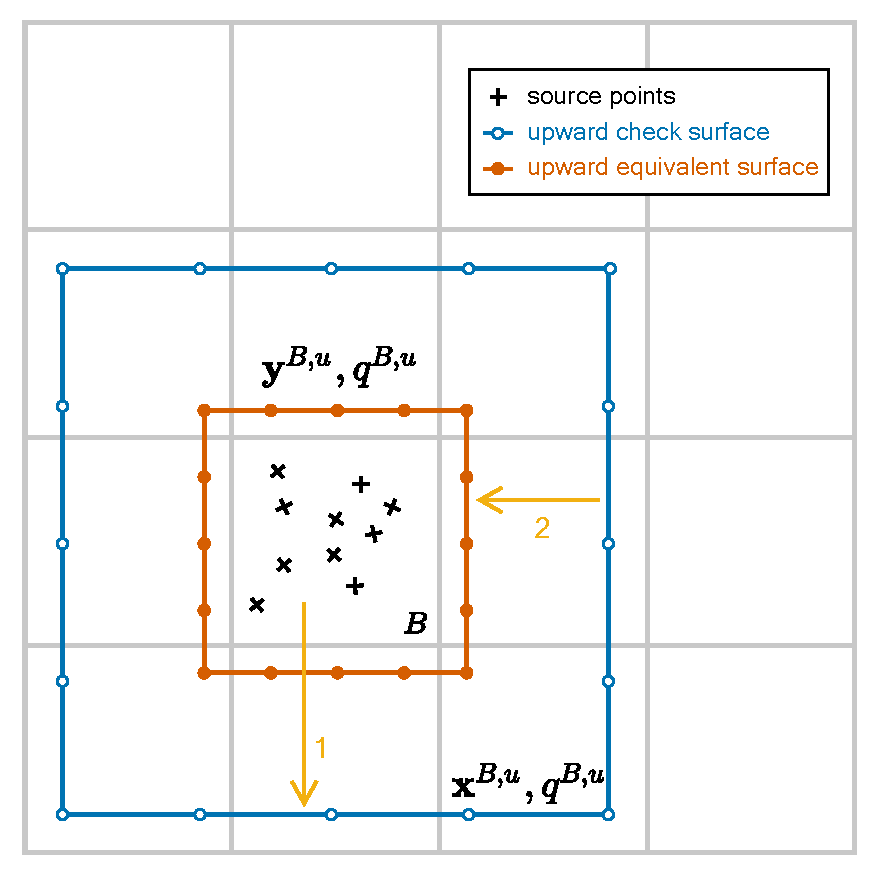
\includegraphics[width=4cm]{../figs/multipole_expansion.pdf}
        \end{tabular}
    \end{center}

\end{frame}
    
%\begin{frame}
%    \frametitle{Coupling Bempp-cl and Exafmm-t}
%
%Let $A$ be the matrix representation of a Galerkin discretised boundary integral operator.
%Let $x$ be any vector. Reformulate $Ax$ as
%
%$$
%Ax = P_{test}^T(G - C)P_{dom}x + Sx
%$$
%
%\begin{itemize}
%    \item $P_{test}$ and $P_{dom}$ highly sparse matrices that map function space coefficients to particle weights at quadrature points.    \item $G$ is black-box operator evaluating particle sums over weights across all quadrature points across all elements.
%    \item $C$ is sparse matrix that contains the particle interactions between neighboring triangles.
%    \item $S$ is sparse matrix containing all singular Galerkin integrals in adjacent elements.
%\end{itemize}
%
%\end{frame}


\begin{frame}
\frametitle{Why large-scale BEM?}

    \vspace{.3cm}

    \begin{minipage}{5cm}
        Solve Poisson-Boltzmann equation
        \begin{align}
            \Delta\phi_1 &= \frac{1}{\epsilon_1}\sum_{k}q_k\delta(\mathbf{r}, \mathbf{r}_k)~\text{in }\Omega_1\nonumber\\
            (\Delta - \kappa^2)\phi_2 &= 0~\text{in }\Omega_2\nonumber
        \end{align}
        Interface conditions on $\Gamma$:
        \begin{align}
            \phi_1 &= \phi_2,\nonumber\\
            \epsilon_1\frac{\partial\phi_1}{\partial\mathbf{n}} &= \epsilon_2\frac{\partial\phi_2}{\partial \mathbf{n}}\nonumber
    \end{align}

    \end{minipage}
    \begin{minipage}{5cm}
        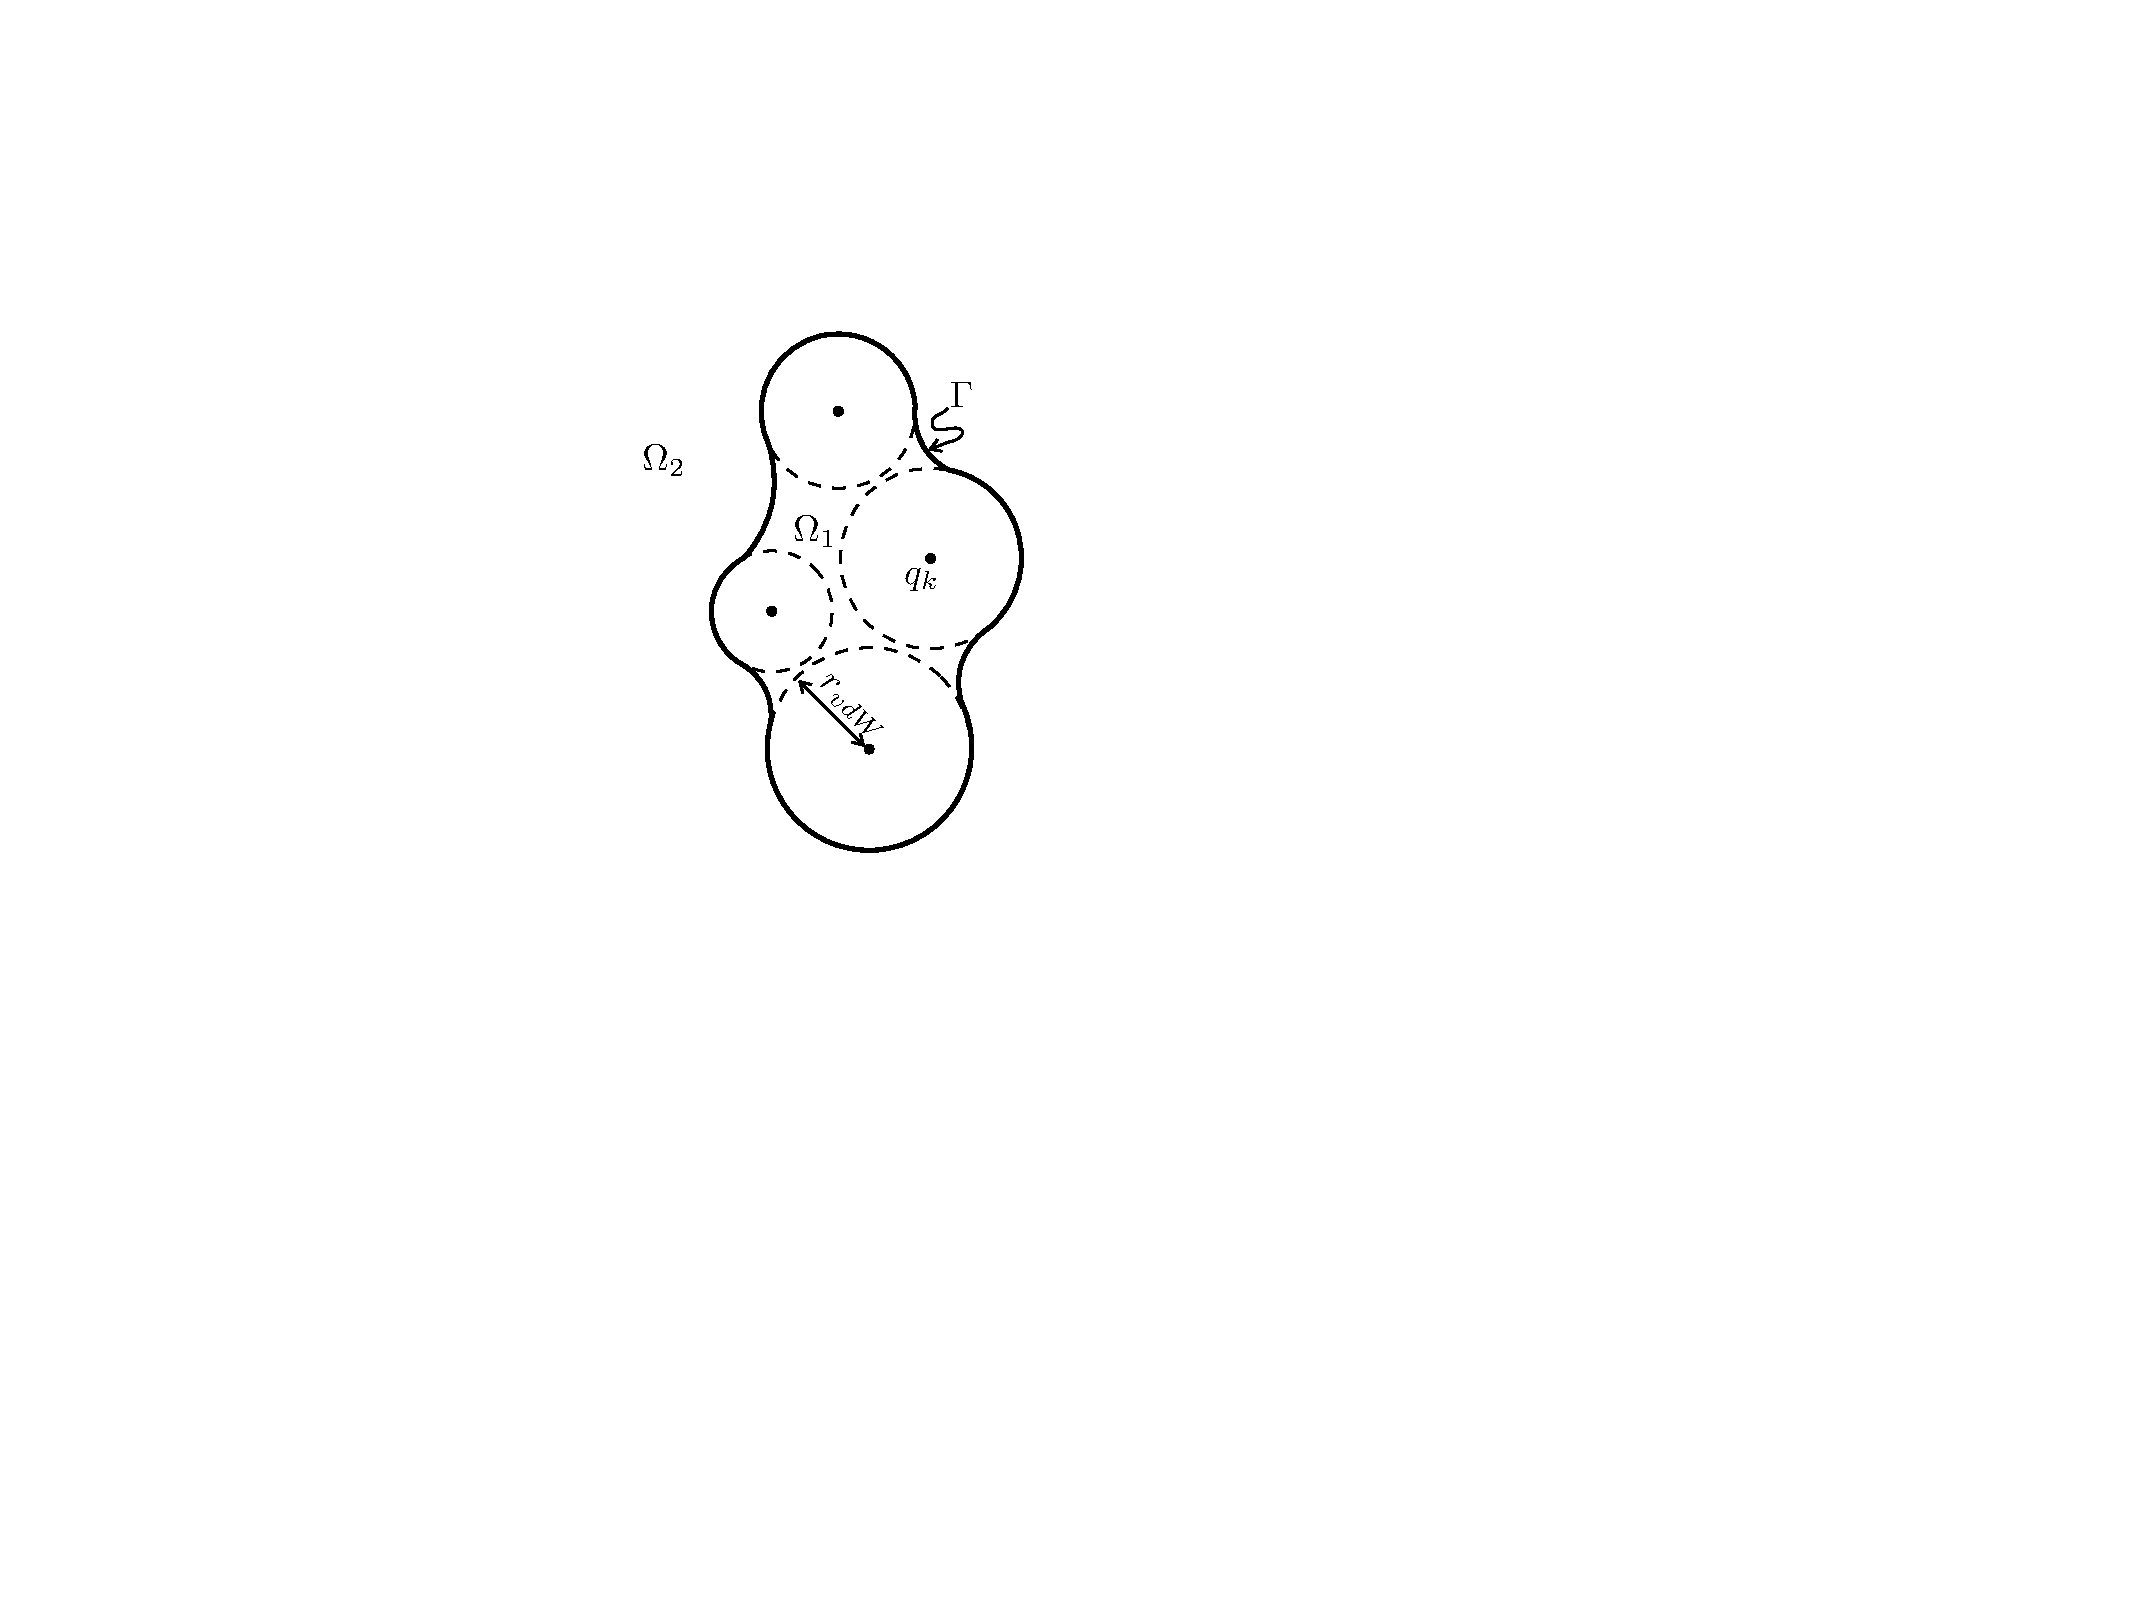
\includegraphics[width=4cm]{../figs/implicit_solvent.pdf}
    \end{minipage}
    Let $\phi_1 = \phi_{reac} + \phi_{coul}$ ($\phi_{coul}$ is potential generated from the point charges only). Then
    want to compute the solvation energy.
    \begin{tcolorbox}
        $$
        \Delta G_{solv}^{polar} = \frac{1}{2}\sum_{k=1}^{N_q}q_k\phi_{reac}(\mathbf{r}_k)
        $$
    \end{tcolorbox}


\end{frame}

\begin{frame}
\frametitle{Exascale FEM/BEM modeling}

\vspace{\baselineskip}

\begin{minipage}{5cm}
    \begin{center}
        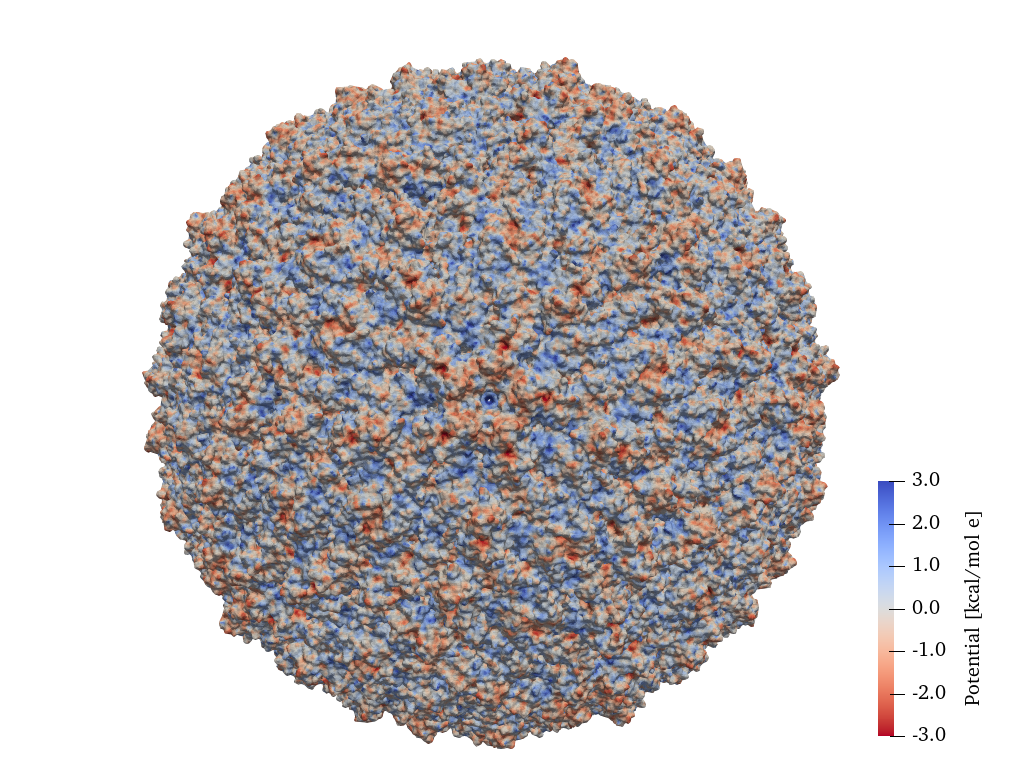
\includegraphics[width=4cm]{../figs/6CO8_potential.png}
    \end{center}
\end{minipage}
\begin{minipage}{5cm}
\small
\begin{itemize}
\item Electrostatic simulation of Zika virus (10m elements) on single compute node\footnotemark
\item Mass-matrix preconditioned single trace formulation.
\item FMM acceleration via ExaFMM.
\end{itemize}
\end{minipage}

\vspace{\baselineskip}

Goal: Full FEM/BEM modelling of complex protein surfaces.\footnotetext{\tiny T. Wang, C. D. Cooper, T. Betcke, L. A. Barba, \textit{High-productivity, high-performance workflow for virus-scale electrostatic simulations with Bempp-Exafmm}, submitted (2021)}

\begin{align*}
\begin{bmatrix}
\epsilon_1 A &  - \epsilon_1 M^T \\
\left(\tfrac12 I + K \right) &  \tfrac{\epsilon_1}{\epsilon_2} V
\end{bmatrix}
\begin{bmatrix}
\vec{\phi}_1 \\
\vec{\lambda}_2
\end{bmatrix}
=
\begin{bmatrix}
\vec{f} \\
0
\end{bmatrix}.
\end{align*}

$A$: FEM matrix, $K$: Double-Layer operator, $V$: Single-Layer operator, $M$: Mass matrix

\begin{tcolorbox}
Want to scale up to billions surface dofs.
\end{tcolorbox}

\end{frame}

\begin{frame}
\frametitle{Deconstructing a BEM operator call}

\begin{minipage}{5cm}
\begin{tcolorbox}
\small
Discrete integral operator evaluation takes the form
$$
Vx = P_{dual}^T(G - C)P_{dom}\overline{x} + S\overline{x}
$$

\begin{itemize}
\item $G$ dense.
\item All other matrices highly sparse.
\end{itemize}
\end{tcolorbox}

\end{minipage}
\begin{minipage}{5cm}
\small
\begin{itemize}
\item $P_{dom/dual}$: Map from domain/dual space cefficients to values at quadrature points
\item $G$ matrix of Green's fct. evaluations at regular Gauss points
\item $C$: Correction matrix containing contribution of $G$ associated with adjacent triangles
\item $S$: Contributions of singular quadrature rule on adjacent triangles
\end{itemize}
\end{minipage}

\vspace{\baselineskip}

\begin{itemize}
\item Parallel fast methods ($H$-matrices/FMM) for $G$.
\item Distributed sparse linear algebra for everything else.
\end{itemize}

\end{frame}

\begin{frame}
    \frametitle{The correction matrix}

    \begin{center}
        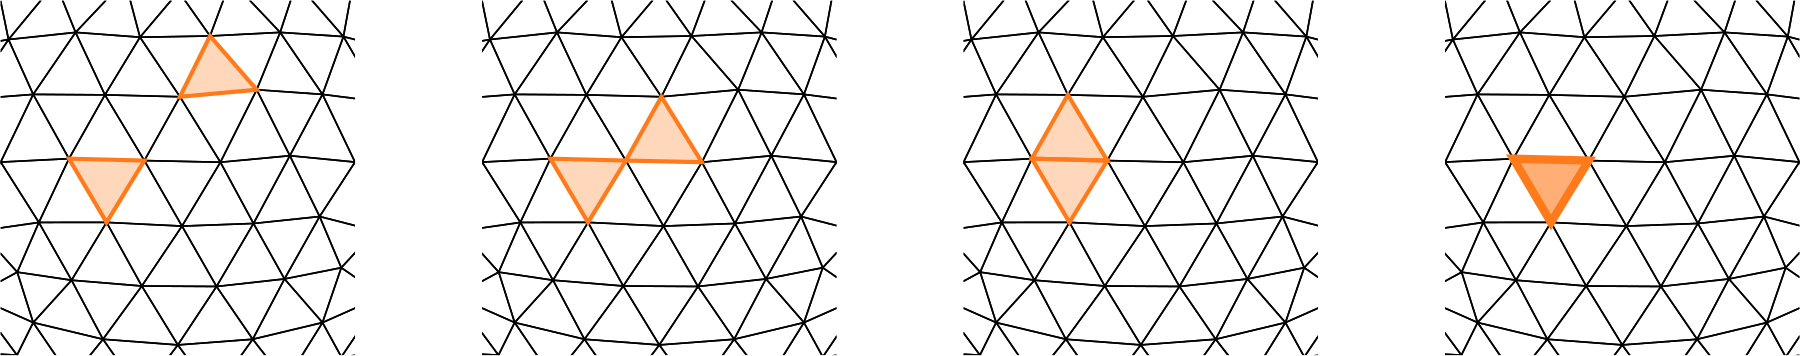
\includegraphics[width=10cm]{../figs/triangles.png}
    \end{center}

    Problem: Any fast code for $G$ also evaluates the near-field.
    Near-field can contain adjacent triangles (singular quadrature rules), and
    non-adjacent triangles (standard triangle Gauss rule).

    \vspace{.5cm}

    The sources and target points in the FMM are arising from the
    non-singular quadrature rule.

    \vspace{.5cm}

    Solution: After FMM evaluation subtract out the regular quadrature rule
    contribution from adjacent triangles and add in the correct singular quadrature
    rule contribution.

\end{frame}



\begin{frame}
\frametitle{Software Technologies}

\begin{tabular}{ll}
\begin{minipage}[t]{6cm}
{\color{blue} Python}
\begin{itemize}
\item Good for higher level logic.
\item Efficient libs for array processing.
\item Performance for complex algorithms in Python (e.g. FMM) difficult\footnotemark.
\end{itemize}
\end{minipage} &
\begin{minipage}[t]{6cm}
{\color{blue} C++}
\begin{itemize}
\item Complex Makefiles.
\item Deployment difficult.
\item C++20 support still patchy.
\end{itemize}
\end{minipage}\\
\begin{minipage}[t]{6cm}
{\color{blue}Python + Code Gen}
\begin{itemize}
\item Most flexible solution.
\item Complex framework.
\item What low-level language to use?
\end{itemize}
\end{minipage} & 
\end{tabular}

\footnotetext{\tiny S. Kailas et. al., \textit{PyExaFMM: an exercise in designing high-performance software with Python and Numba}, to be submitted}

\end{frame}

\begin{frame}
\frametitle{Along came Rust}
\begin{minipage}{5cm}
\begin{itemize}
\item Modern language design.
\item Great tooling.
\item Compile time safety guarantees.
\item Simple deployment.
\item Python integration trivial.
\end{itemize}
\end{minipage}
\begin{minipage}{5cm}
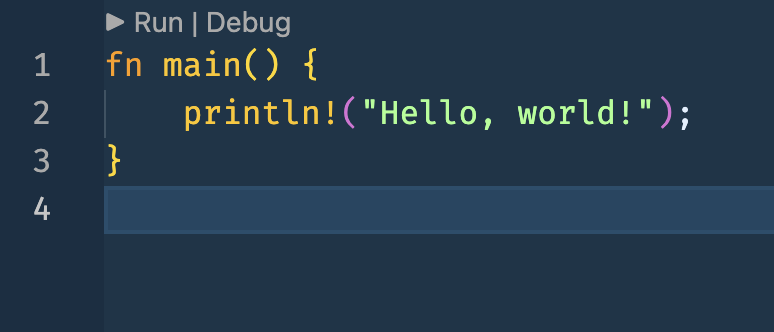
\includegraphics[width=5cm]{../figs/rust_hello}
\end{minipage}

\vspace{2\baselineskip}

\begin{tcolorbox}
Design a set of micro-libraries in Rust that can be easily composed into large parallel FEM/BEM applications.
\end{tcolorbox}

\end{frame}

\begin{frame}
\frametitle{A set of micro-libraries in Rust}

	
	{Blue}: Finished or in work. {Red}: In planning
	
	{\small
	\begin{center}
	
	\begin{tabular}{|l|l|}
	\hline
	{\color{blue}tree} & Fast distributed octree management\\
	\hline
	{\color{blue}compression} & Linear algebra tools for low-rank compression\\
	\hline
	{\color{red}field} & Field translation operators\\
	\hline
	{\color{blue}green-kernel} & Direct evaluation of Green's functions\\
	\hline
	{\color{blue}quadrature} & Collection of quadrature rules\\
	\hline
	{\color{blue}element} & Finite element definitions\\
	\hline
	{\color{red}grid} & Distributed management of surface grids\\
	\hline
	{\color{red}fmm} & High-Level distributed FMM loops\\
	\hline
	{\color{red}surface-diff-op} & Distributed assembly of surface differential operators\\
	\hline
	{\color{red}bempp} & High-Level distributed BEM interface\\
	\hline
	
	\end{tabular}
	
		
	\end{center}
	}
	\begin{itemize}
	\item All libraries independent projects
	\item MPI support where necessary
	\item C interface + Python bindings for most functionality
	\item From October team of 1 PhD, 1 Postdoc + Research Software Engineers
	
	\end{itemize}
	
\end{frame}

\begin{frame}
\frametitle{rusty-tree}

\begin{minipage}{5cm}
\begin{itemize}
\item Modeled on Sundar et. al\footnotemark
\item Distributed load-balancing, 2:1 refinement
\item Full Python interface
\item Can use Rust or Python MPI communicator
\end{itemize}
\end{minipage}
\begin{minipage}{5cm}
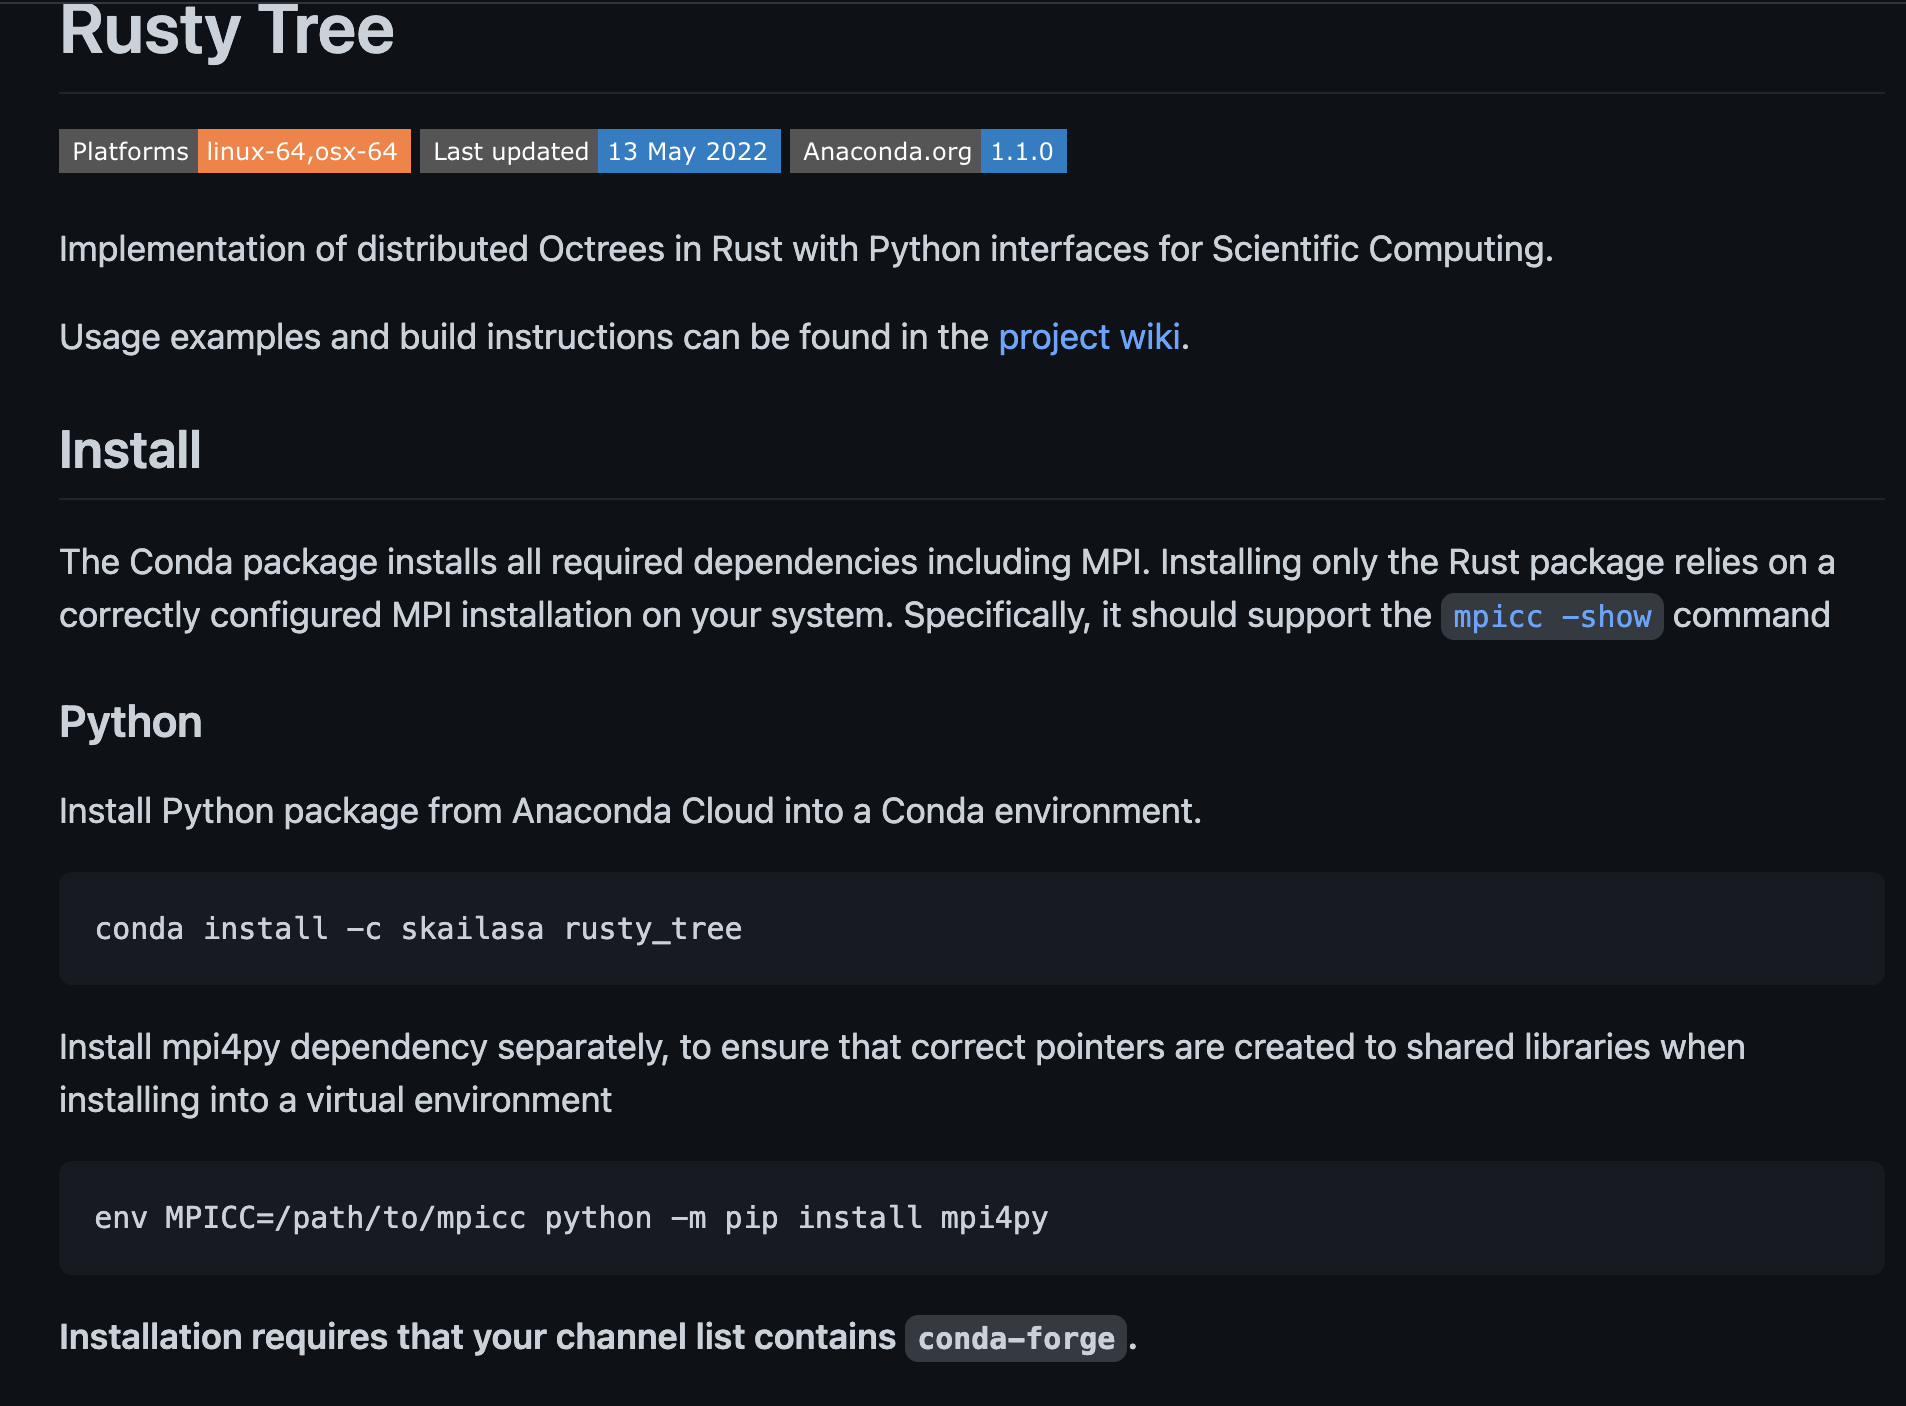
\includegraphics[width=5cm]{../figs/rusty_tree}
\end{minipage}

\footnotetext{\tiny H. Sunar, R. S. Sampath, G. Biros, \textit{Bottom Up Construction and 2:1 Balance Refinement of Linear
Octrees in Parallel}, 30 (2008, pp. 2675 - 2708}

\end{frame}

\begin{frame}
\frametitle{rusty-compression}
\begin{minipage}{5cm}

\begin{tcolorbox}
Low-rank compression
$$
A\approx UV^H
$$

$A\in\mathbb{C}^{m\times n}$, $U\in\mathbb{C}^{m\times k}$, $V\in\mathbb{C}^{k\times n}$.
\end{tcolorbox}
\end{minipage}
\begin{minipage}{5cm}
\begin{itemize}
\item Dense QR, SVD decomposition
\item Interpolative decompositions
\item Randomized low-rank decompositions
\end{itemize}
\end{minipage}

\vspace{2\baselineskip}

\begin{itemize}
\item Required for algebraic compression of translation operators.
\item Currently uses Blas/Lapack/ndarray.
\item Plan to rebase on new linear algebra core.
\end{itemize}
\end{frame}

\begin{frame}
\frametitle{rusty-element}

\begin{center}
\begin{tabular}{cc}
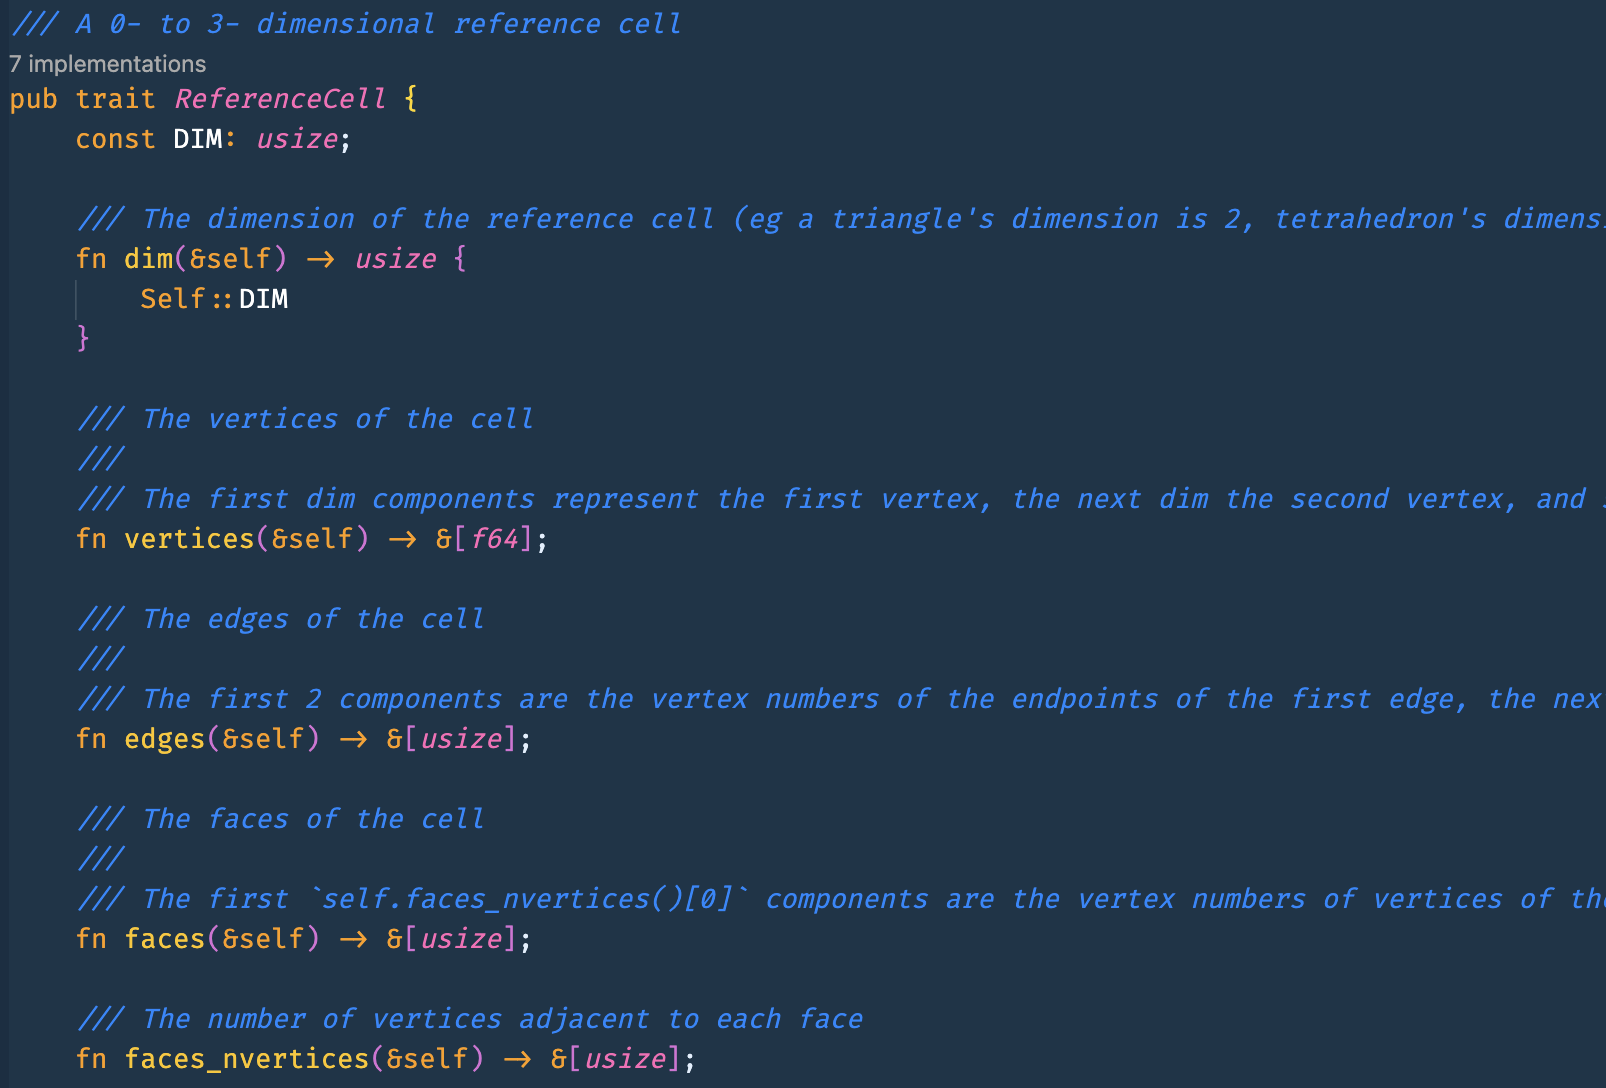
\includegraphics[width=5cm]{../figs/rusty_element} &
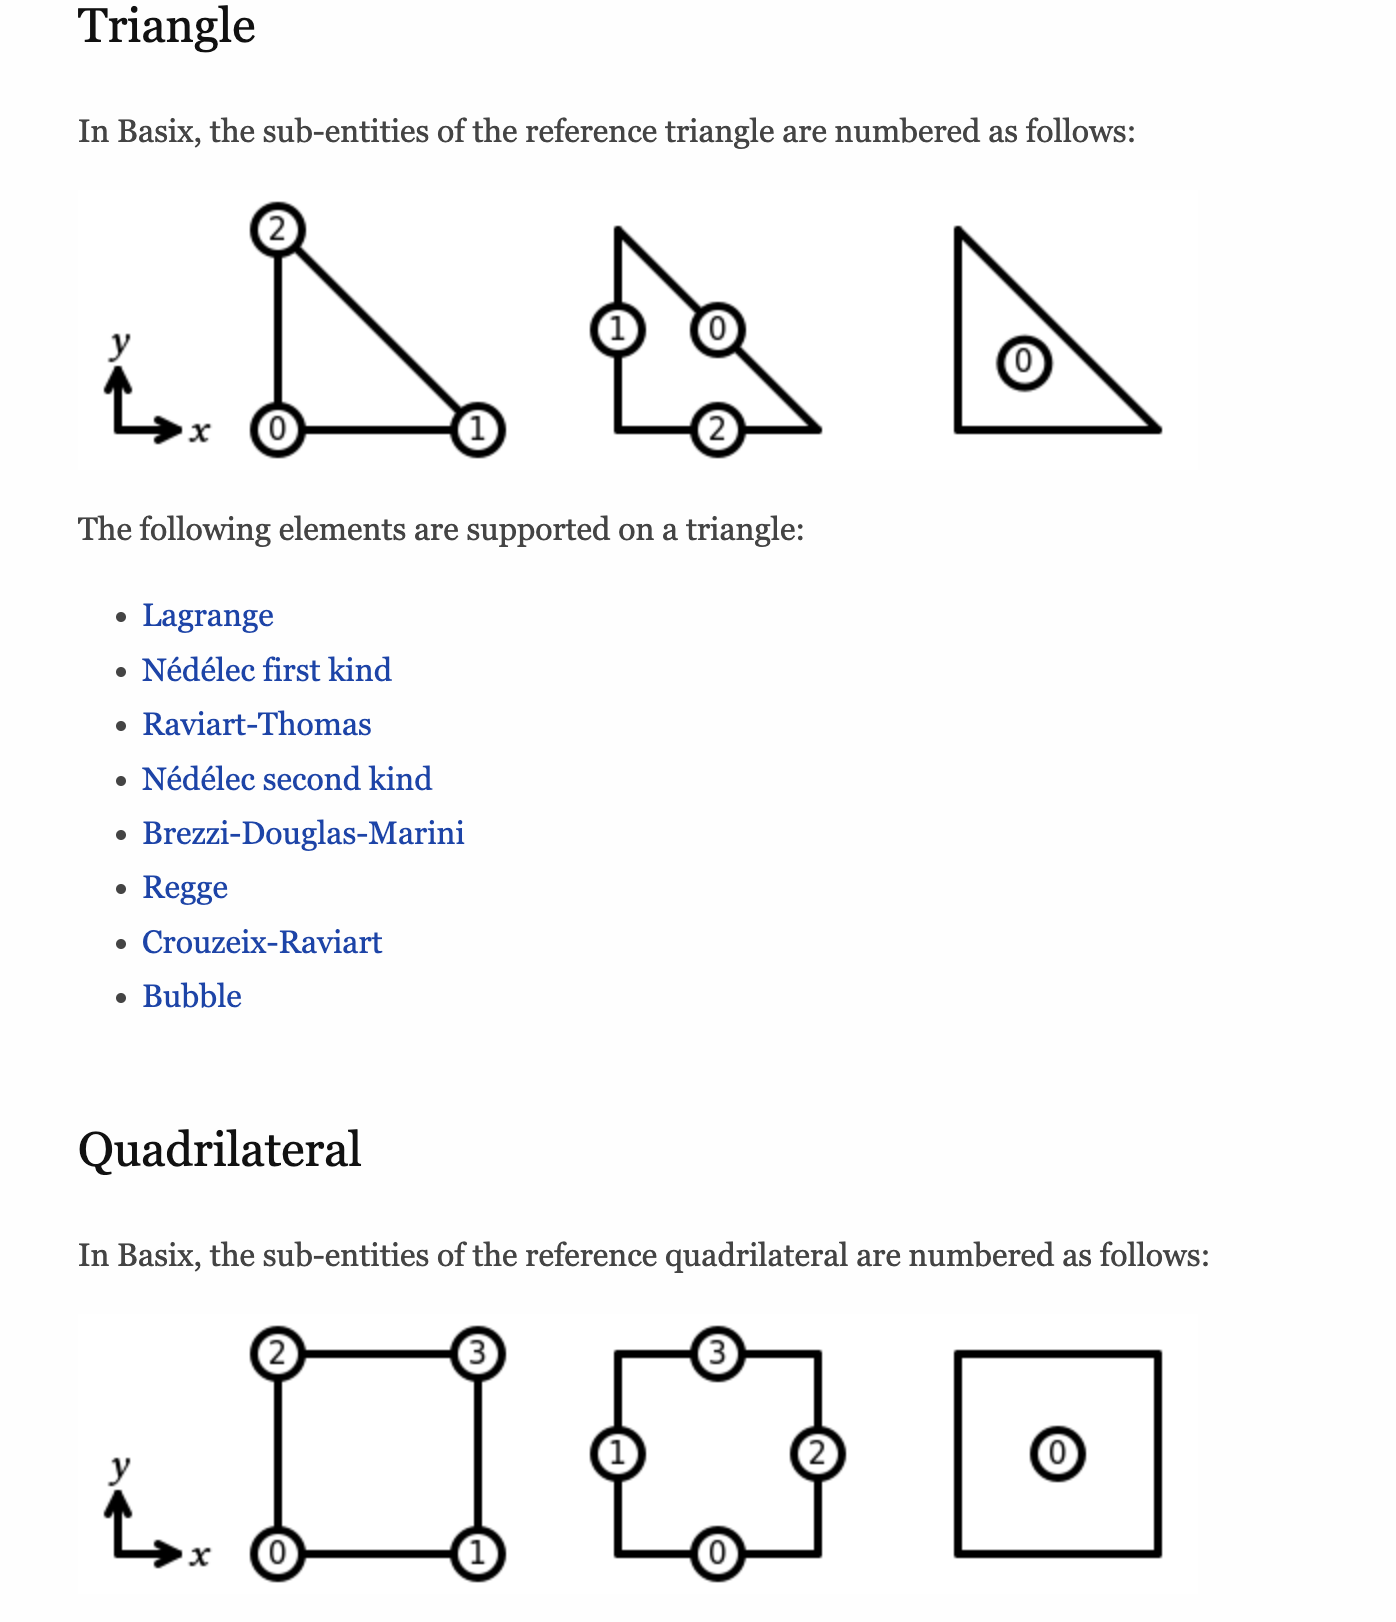
\includegraphics[width=4cm]{../figs/basix_elements}\\
Reference Cell Trait & {\small Basix elements}
\end{tabular}
\end{center}

\begin{itemize}
\item Modeled on Basix (FeniCS finite element evaluation library).
\item Generic interface and implementation of element definitions.
\item Support for higher order triangular and quadrilateral elements.
\item Separate from grid library (grid library does data distribution and
iteration, rusty-element provides element information).
\end{itemize}

\end{frame}

\begin{frame}
\frametitle{Householder - A new linear algebra kernel in Rust}

\begin{center}
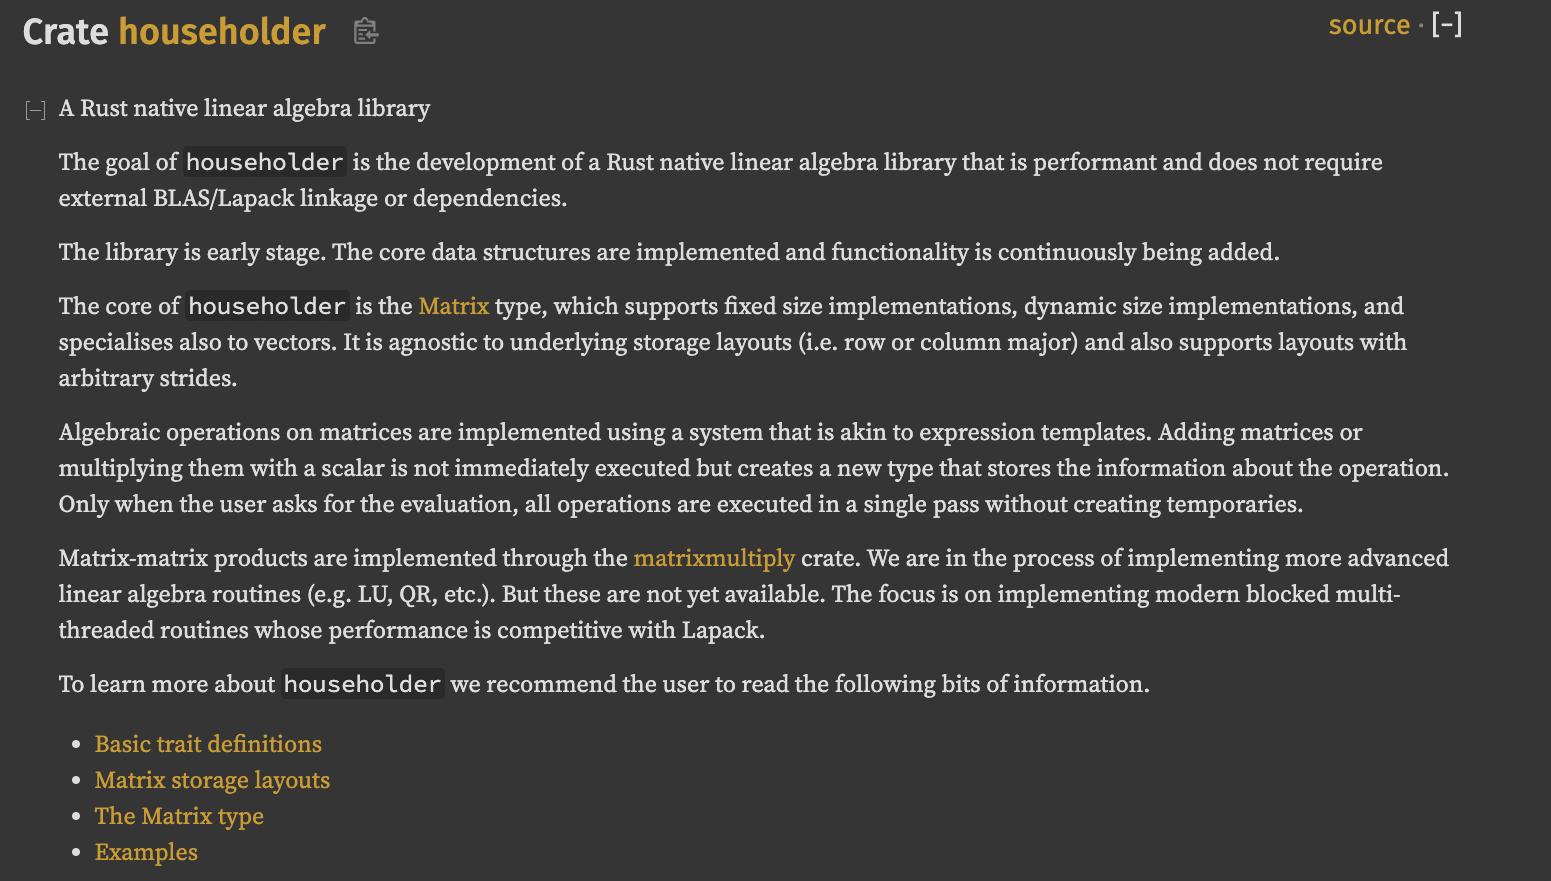
\includegraphics[width=8cm]{../figs/householder}
\end{center}

\begin{itemize}
\item New dense/sparse linear algebra kernel in Rust.
\item Based on Rust implementation of expression templates (similar to C++ eigen).
\item Supported by ARCHER2 eSAFE funding.
\end{itemize}

\end{frame}

\begin{frame}
\frametitle{Diving into Rust with Householder}

\begin{itemize}
\item Matrix traits
\item Mutable and immutable access
\item Basic data containers (vectors and slices)
\item Reference types and lifetimes
\item A generic matrix structure
\item Documentation and unit tests
\end{itemize}

\end{frame}

\begin{frame}
\frametitle{The Rust Scientific Computing ecosystem}

{\tiny

\begin{tabular}{cc}
\begin{minipage}[t]{5cm}
{\color{blue} Core utilities}
\begin{itemize}
\item Num - Traits and utility routines for floating point types.
\item Cauchy - A complex scalar type library (uses Num).
\item approx - Unit test routines for floating point types.
\item Serde - Serialization library.
\end{itemize}
\end{minipage} & 
\begin{minipage}[t]{5cm}
{\color{blue}Parallelization}
\begin{itemize}
\item rsmpi - MPI Interface for Rust.
\item Rayon - Fork/Join threading, parallel loops and iterators.
\item async/await (Tokio, etc.) - frameworks for asynchroneous execution.
\end{itemize}
\end{minipage}\\
\begin{minipage}[t]{5cm}
{\color{blue} Linear Algebra/Machine Learning}
\begin{itemize}
\item ndarray - multidimensional array type in Rust.
\item nalgebra - Rust linear algebra library with Lapack bindings.
\item householder - Early stages linear algebra library.
\item Linfa - Native machine learning in Rust.
\item tensorflow - Rust bindings to tensorflow.
\item petsc-rs - Rust bindings for Petsc.
\end{itemize}
\end{minipage} &
\begin{minipage}[t]{5cm}
{\color{blue} Language bindings}
\begin{itemize}
\item PyO3 - Binding complex Rust types to Python.
\item maturin - Simple tools to wrap Rust C API bindings with Python cffi.
\item Any language that supports C bindings can talk to Rust easily.
\end{itemize}
\end{minipage}

\end{tabular}

}

\vspace{\baselineskip}

\begin{tcolorbox}
Still lots of moving parts in the ecosystem but an enormous amount of development happening.
\end{tcolorbox}

\end{frame}


\begin{frame}
\frametitle{Some final messages}
\begin{itemize}
\item Using Python + JIT (e.g. Numba) works well for simple array oriented algorithms. More problematic for complex algorithms.
\item We are at the start of a multi-year journey to develop very large-scale integral equation solvers in Rust.
\item Rust is ready to be looked at by Scientific Computing Community (though far away from the level of maturity of the C++ ecosystem)
\item Rust makes little sense when legacy C++ code exists or there is need for heterogeneous compute with SyCL or Cuda.
\item But consider and evaluate Rust if you start a completely new project.
\end{itemize}
\end{frame}


\end{document}

\begin{frame}[fragile]{Numba acceleration}

\begin{columns}[T]
\begin{column}{.48\textwidth}
\begin{center}
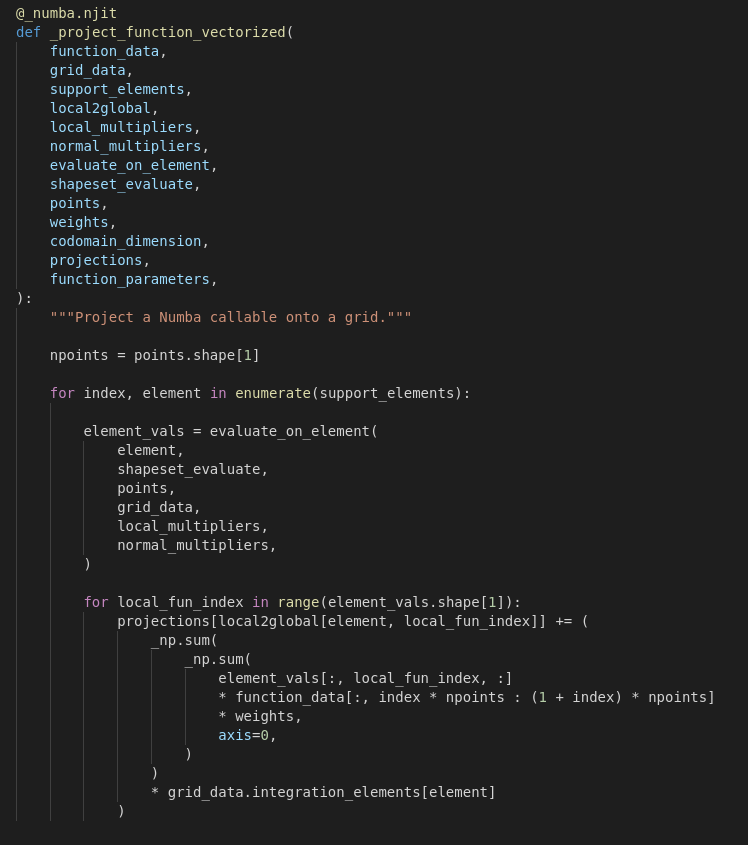
\includegraphics[width=6cm]{../figs/grid_fun_discretise.png}
\end{center}
\end{column}%
\hfill%
\begin{column}{.48\textwidth}

\vspace{1cm}

\begin{itemize}
    \item Numba just-in-time compiles Python functions to machine code (using LLVM).
    \item Executable code independent of the Python interpreter.
    \item Allows simple loop-based threading.
    \item Most Python features and many Numpy features supported.
\end{itemize}

\end{column}%
\end{columns}

\end{frame}

\begin{frame}{Kernel based programming with OpenCL}
\begin{minipage}{5cm}
\begin{center}
    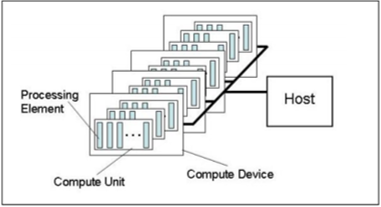
\includegraphics[width=5cm]{../figs/opencl_overview.png}
\end{center}
\end{minipage}
\begin{minipage}{5cm}
\begin{small}
\begin{itemize}
\item Heterogeneous compute model
\item MIMD/SIMD/SIMT support
\item C99 based kernel language
\item Current version 2.2
\item OpenCL drivers by Intel, AMD, Nvidia plus open-source
\end{itemize}
\end{small}
\end{minipage}
\begin{minipage}{5cm}
\begin{small}
\begin{itemize}
\item Each device consists of compute units (e.g. CPU cores) and processing elements (e.g. SIMD lanes)
\item Work items arranged into work groups
\item Memory synchronization only inside a workgroup
\item Excellent Python support through PyOpenCL by Andreas Kloeckner
\end{itemize}
\end{small}
\end{minipage}
\begin{minipage}{5cm}
\begin{center}
    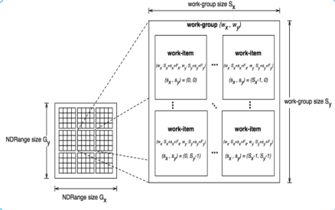
\includegraphics[width=5cm]{../figs/cl_workgroups.png}
\end{center}
\end{minipage}

\end{frame}



\begin{frame}[fragile]{Compute kernels for regular integrals}

{\footnotesize
\begin{lstlisting}[language=C]

__kernel void kernel_function(...){

  size_t testIndex = testIndices[gid[0]];
  size_t trialIndex = trialIndices[gid[1]];

  // Compute geometric data
  
  // Evaluate all integral contributions for test/trial pair
  
  // Sum into global matrix if test/trial pair not adjacent

}

\end{lstlisting}
}
\begin{tcolorbox}
    \begin{itemize}
        \item Compute kernels are JIT-compiled during Python execution by the OpenCL driver
        \item On CPUs one test triangle coalesced with 4/8/16 trial triangles to efficiently target SIMD lanes.
        \item A typical computation launches millions of kernels
    \end{itemize}
\end{tcolorbox}

\end{frame}

\begin{frame}
	\frametitle{Performance}
	
	\begin{center}
	\begin{tabular}{cc}
		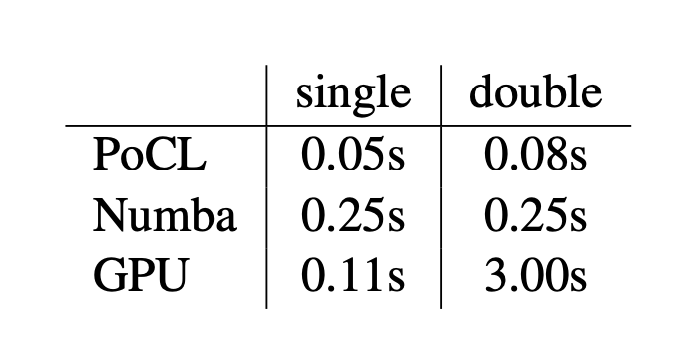
\includegraphics[width=5cm]{../figs/cpu_vs_gpu.png} &
		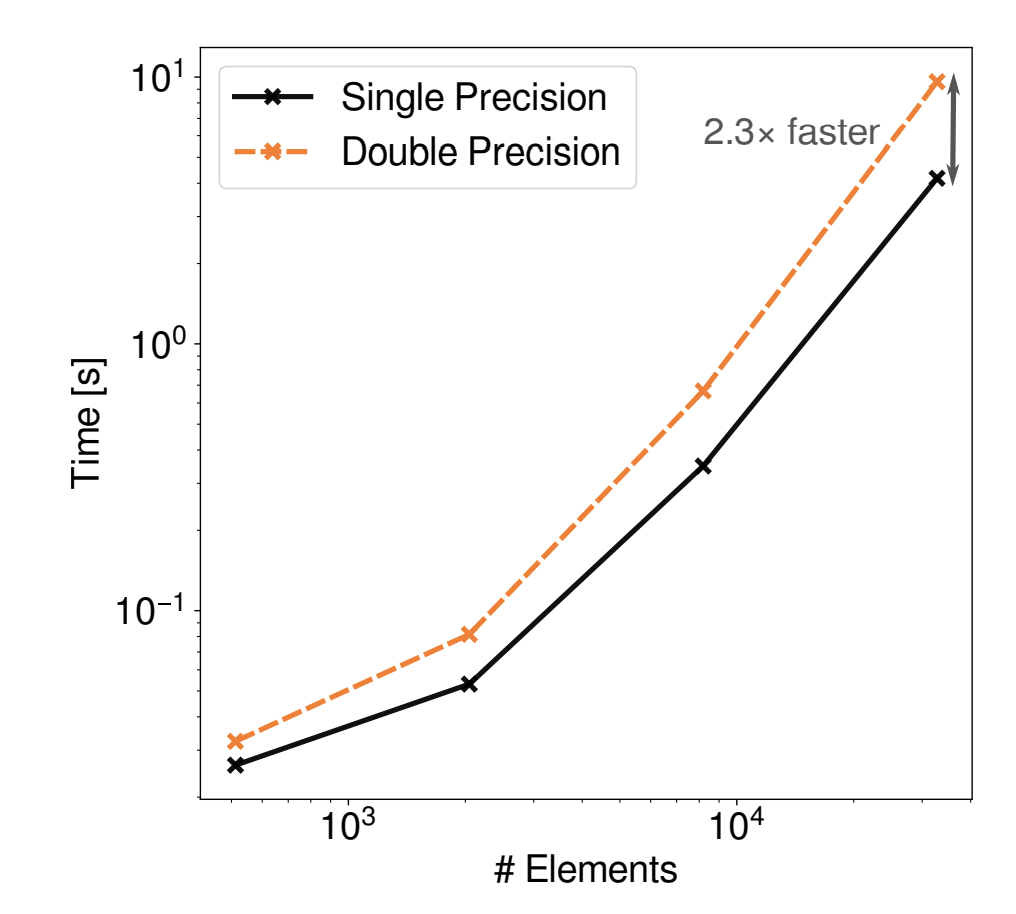
\includegraphics[width=5cm]{../figs/single_vs_double.png}\\
		\begin{minipage}{5cm}
			Boundary op. assembly times (2048 elem)
		\end{minipage} &
		\begin{minipage}{5cm}
			Single vs double precision assembly on CPU
		\end{minipage}
	\end{tabular}
	\end{center}
\end{frame}
		
		
\begin{frame}
	\frametitle{Am I finally happy?}
	
	\begin{itemize}
		\item {\color{blue} Python + Numba + OpenCL powerful environment for multitude of tasks}
		\item {\color{blue} Can make use of modern CPU/GPU features}
		\item {\color{blue} New code much faster than our old C++ code}
	\end{itemize}
	
	\vspace{\baselineskip}
	
	But...
	
	\begin{itemize}
		\item {\color{red} Need to deal with OpenCL drivers from different vendors}
		\item {\color{red} Numba JIT not sufficiently performant on CPUs to replace OpenCL}
		\item {\color{red} Thousands of lines of low-level OpenCL C99 kernel code}
		\item {\color{red} Latency issues for pure Python operations}
		\item {\color{red} Numba not a good model for very complex algorithms}
	\end{itemize}
		
	
\end{frame}

\begin{frame}

	\frametitle{What now?}
	
	\begin{itemize}
	\item Python with C++ is complex with cumbersome build systems and terrible dependency management
	\item Python with JIT compilation works for certain tasks but not algorithms with complex structures. Optimising
		the code can become complicated.
	\item We need to address the Exascale challenge.
	\end{itemize}
	
\end{frame}

\begin{frame}
\frametitle{Why exascale BEM?}

\begin{minipage}{5cm}
    \begin{center}
        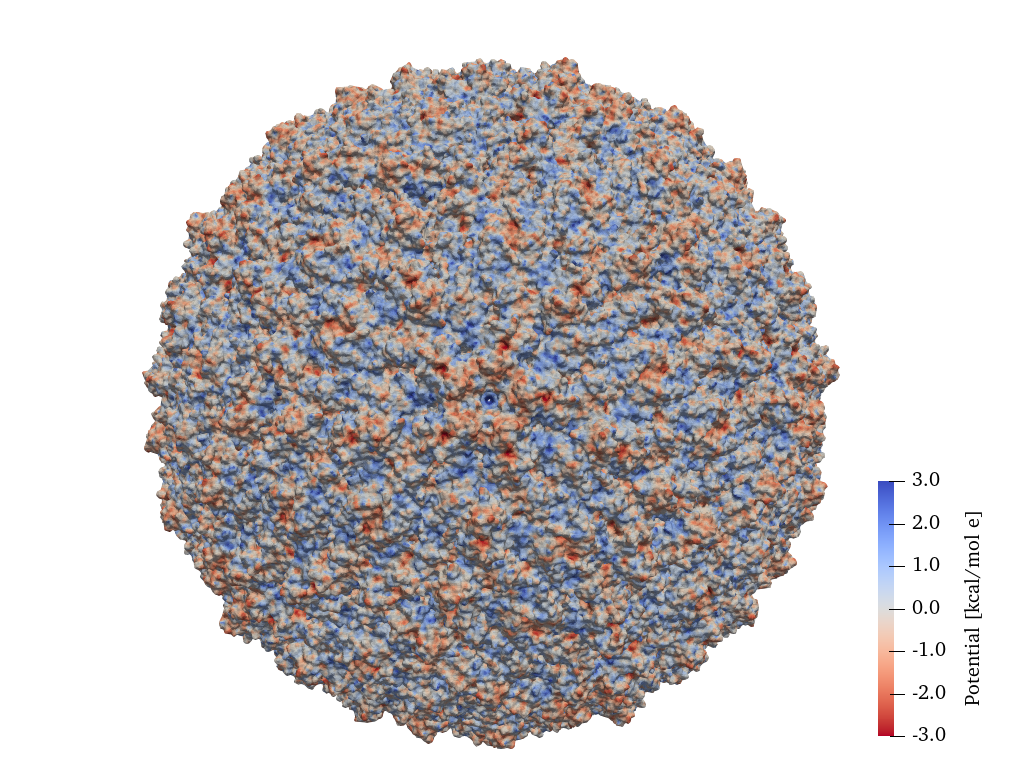
\includegraphics[width=5cm]{../figs/6CO8_potential.png}
    \end{center}
\end{minipage}
\begin{minipage}{5cm}
\begin{itemize}
\item Joint with L. Barba, C. Cooper, T. Wang
\item Poisson-Boltzmann equation
\item 10m elements on single workstation
\item Bempp-cl + Exafmm
\end{itemize}
\end{minipage}

\vspace{\baselineskip}

\begin{tcolorbox}
Need to scale up to 100m - 1b surface elements plus interior volume discretisation
\end{tcolorbox}

\end{frame}

\begin{frame}
	\frametitle{Some exascale challenges}
	
	\begin{itemize}
	\item Code should be highly portable and scalable from Laptop to cluster.
	\item Heterogeneous compute capabilities.
	\item $\mathcal{O}(n)$ complexity algorithms.
	\item High-order methods to generate enough compute intensity.
	\end{itemize}
	
\end{frame}

\begin{frame}
	\frametitle{Component libraries}
	
	We have in {\color{red}planning} or {\color{blue}active development} the following component libraries
	
	{\small
	\begin{center}
	
	\begin{tabular}{|l|l|}
	\hline
	{\color{blue}octree} & Fast distributed octree management\\
	\hline
	{\color{blue}compression} & Linear algebra tools for low-rank compression\\
	\hline
	{\color{red}field} & Field translation operators\\
	\hline
	{\color{blue}green-kernel} & Direct evaluation of Green's functions\\
	\hline
	{\color{red}integration} & Collection of quadrature rules\\
	\hline
	{\color{red}grid} & Distributed management of surface grids\\
	\hline
	{\color{red}fmm} & High-Level distributed FMM loops\\
	\hline
	{\color{red}surface-diff-op} & Distributed assembly of surface differential operators\\
	\hline
	{\color{red}bempp} & High-Level distributed BEM interface\\
	\hline
	
	\end{tabular}
	
		
	\end{center}
	}
	\begin{itemize}
	\item All libraries independent projects
	\item MPI support where necessary
	\item C interface + Python bindings for most functionality
	\item From October team of 1 PhD, 1 Postdoc + Research Software Engineers
	
	\end{itemize}

	
\end{frame}
	


\begin{frame}
	\frametitle{We do Rust}
	
	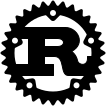
\includegraphics[width=2cm]{../figs/rust_logo.png}
	
	
	\begin{itemize}
	\item We decided to use Rust as we have no existing legacy code.
	\item Rust is modern, low-level systems language with excellent dependency management
	         and no more need for complex build scripts.
	 \item Strong industry support + growing HPC community.
	 \item Ideal for low-level library development.
	 \item Great tooling + Python integration.
	 \end{itemize}
	
\end{frame}

\end{document}

\begin{frame}
\frametitle{Conclusions}

	\begin{itemize}
	\item We are at the start of exciting new code developments.
	\item Please share your opinions with us!
	
	\end{itemize}
	
\vspace{2\baselineskip}	

\begin{tcolorbox}Head to the talk by Maria Ignacia Fierro-Piccardo to
see some of our work on {\color{red}Maxwell preconditioning.} \\ 
{\color{blue}Monday, 4pm, Green 3}\end{tcolorbox}


\end{frame}



%\begin{frame}
%    \frametitle{Poisson-Boltzmann for virus simulations}
%
%    \vspace{.3cm}
%
%    \begin{minipage}{5cm}
%        Solve Poisson-Boltzmann equation
%        \begin{align}
%            \Delta\phi_1 &= \frac{1}{\epsilon_1}\sum_{k}q_k\delta(\mathbf{r}, \mathbf{r}_k)~\text{in }\Omega_1\nonumber\\
%            (\Delta - \kappa^2)\phi_2 &= 0~\text{in }\Omega_2\nonumber
%        \end{align}
%        Interface conditions on $\Gamma$:
%        \begin{align}
%            \phi_1 &= \phi_2,\nonumber\\
%            \epsilon_1\frac{\partial\phi_1}{\partial\mathbf{n}} &= \epsilon_2\frac{\partial\phi_2}{\partial \mathbf{n}}\nonumber
%    \end{align}
%
%    \end{minipage}
%    \begin{minipage}{5cm}
%        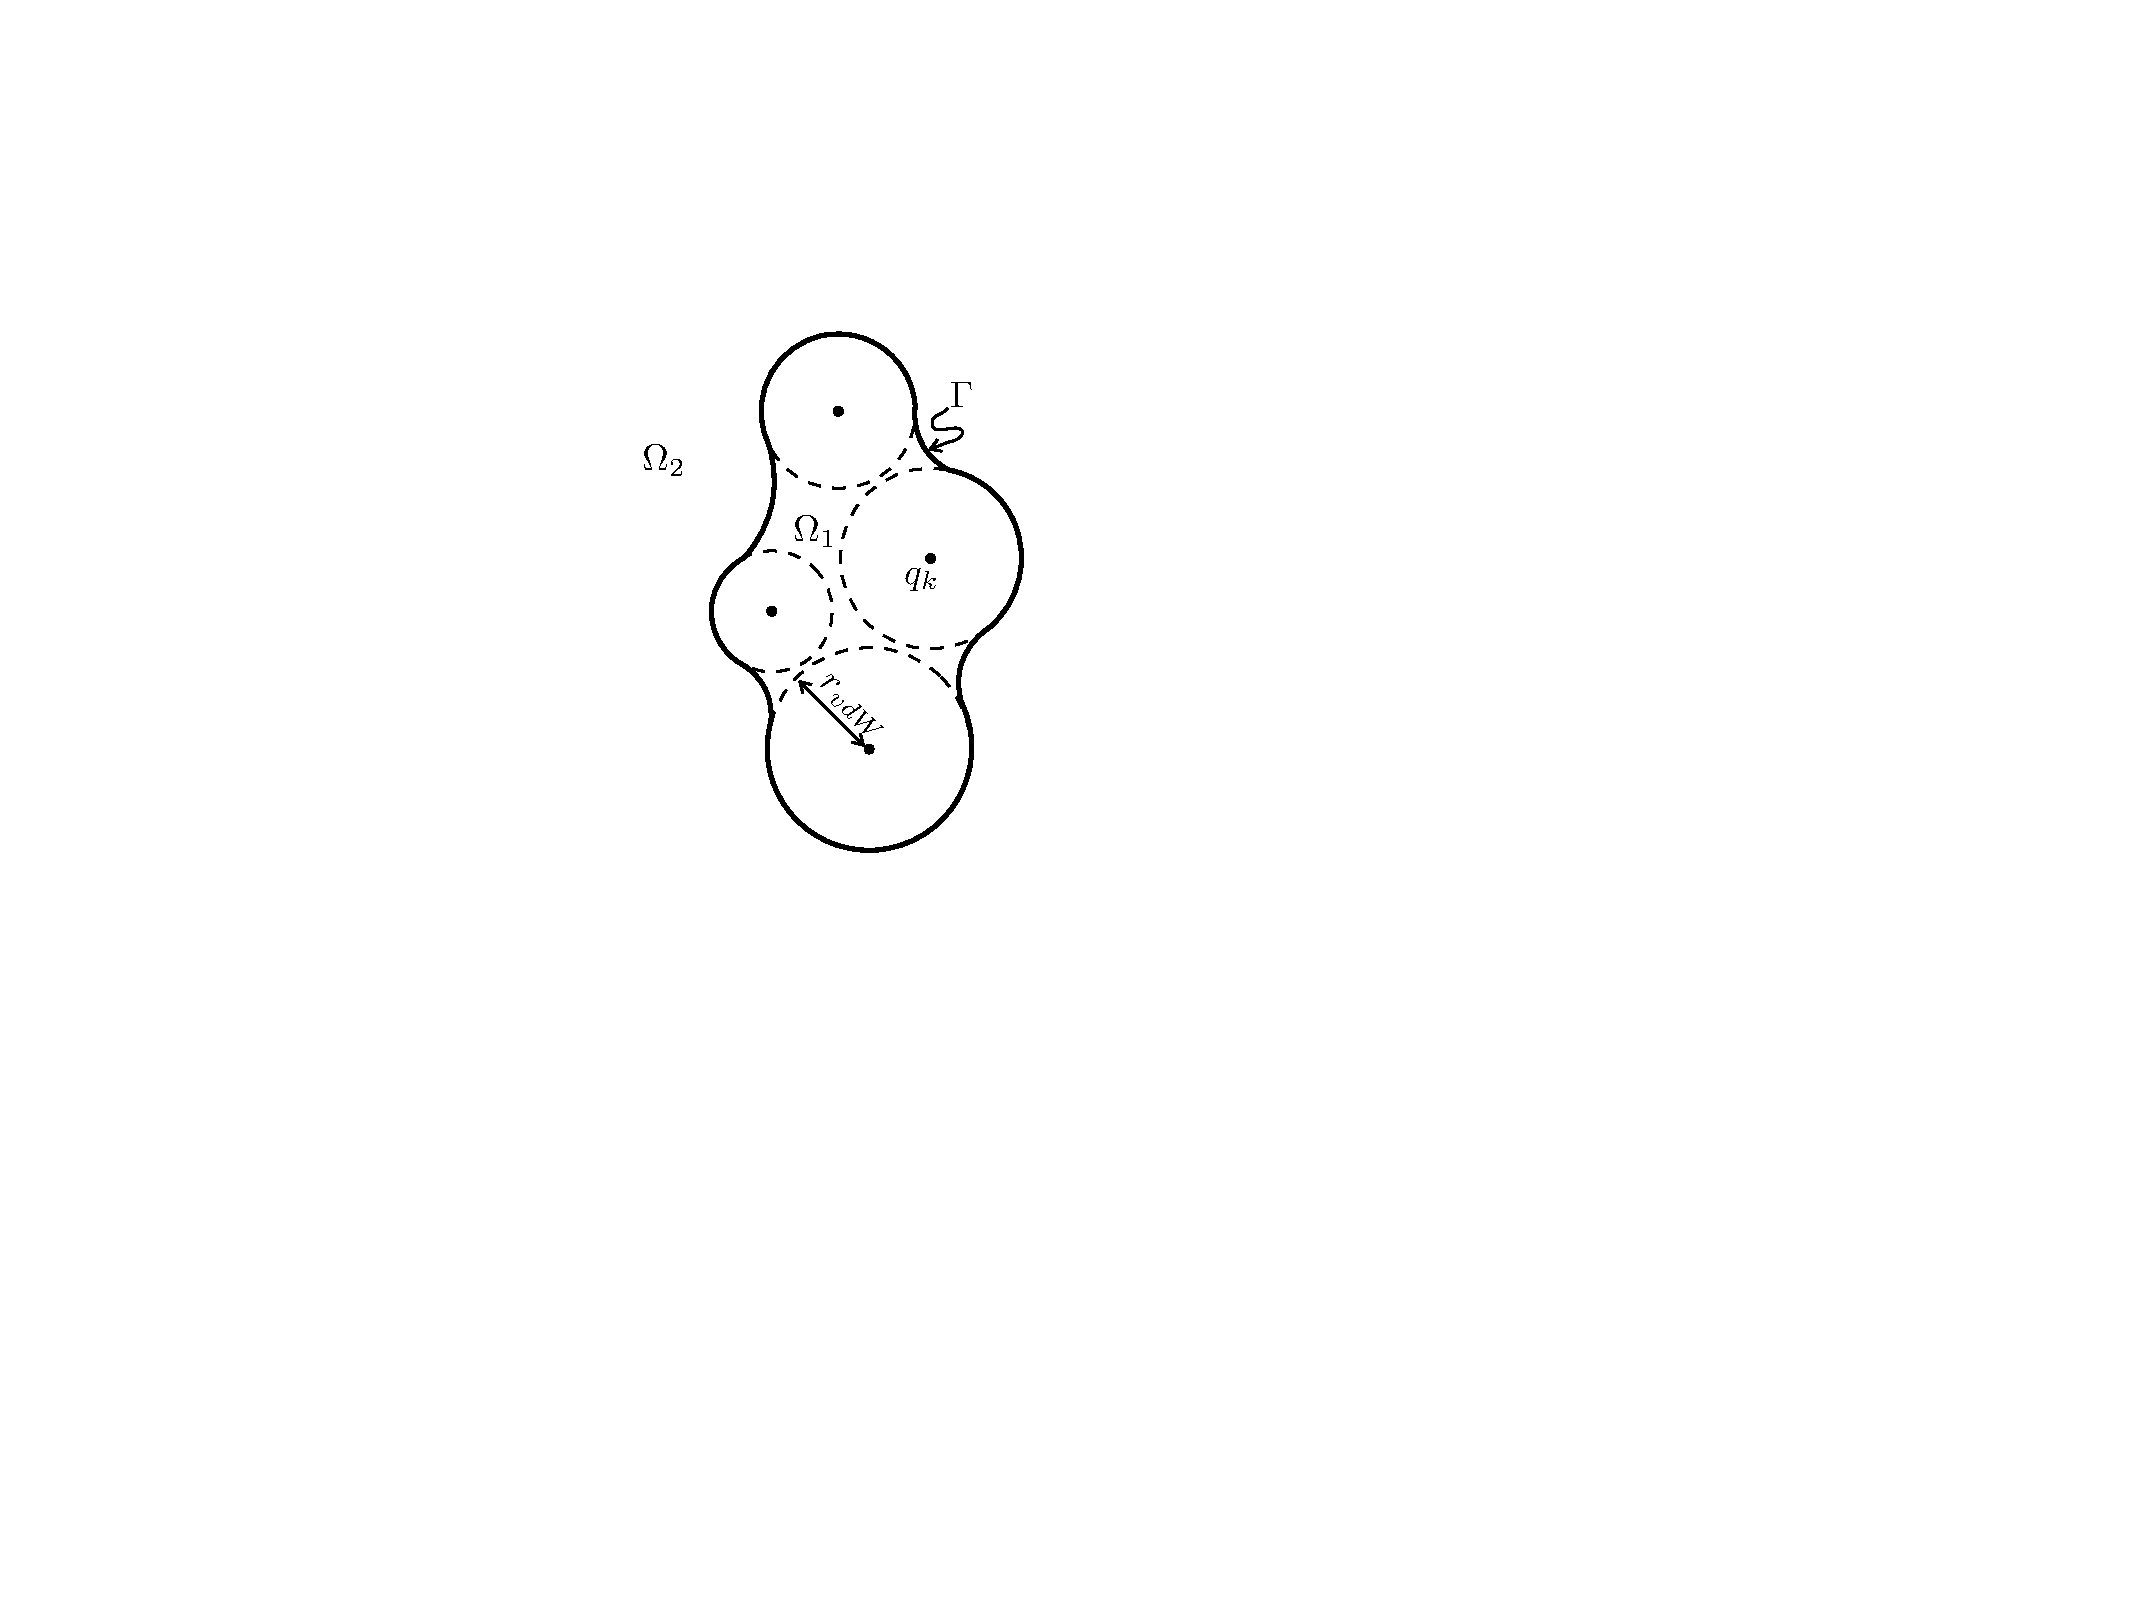
\includegraphics[width=4cm]{../figs/implicit_solvent.pdf}
%    \end{minipage}
%    Let $\phi_1 = \phi_{reac} + \phi_{coul}$ ($\phi_{coul}$ is potential generated from the point charges only). Then
%    want to compute the solvation energy.
%    \begin{tcolorbox}
%        $$
%        \Delta G_{solv}^{polar} = \frac{1}{2}\sum_{k=1}^{N_q}q_k\phi_{reac}(\mathbf{r}_k)
%        $$
%    \end{tcolorbox}
%
%\end{frame}
%
%\begin{frame}
%    \frametitle{Boundary Integral Formulation}
%
%    Exterior field formulation\footnote{Lu et. al., Proc. Natl. Acad. Sci. USA 103 (51) (2006) 19314-19319}
%    
%\begin{align}
%    &\begin{multlined}[t][0.48\textwidth] \frac{\phi_{2,\Gamma}}{2}\left(\frac{\epsilon_1}{\epsilon_2}+1\right) - \left(K_Y^\Gamma - \frac{\epsilon_1}{\epsilon_2}K_L^\Gamma\right)(\phi_{2,\Gamma}) \\
%    + \left(V_Y^\Gamma - V_L^\Gamma\right)\left( \frac{\partial}{\partial \mathbf{n}} \phi_{2,\Gamma} \right) = \sum_{k=0}^{N_q}  \frac{q_k}{4\pi\epsilon_2|\mathbf{r}_{\Gamma} - \mathbf{r}_k|}
%    \end{multlined} \nonumber \\
%    &\begin{multlined}[t][0.48\textwidth] -\frac{\epsilon_1}{\epsilon_2}\left(W_Y^\Gamma - W_L^\Gamma\right)(\phi_{2,\Gamma}) +  \frac{1}{2}\frac{\phi_{2,\Gamma}}{\partial\mathbf{n}}\left(1+\frac{\epsilon_1}{\epsilon_2}\right) \\
%    + \left(\frac{\epsilon_1}{\epsilon_2}K_Y^{\prime\Gamma} - K_L^{\prime\Gamma}\right)\left( \frac{\partial}{\partial \mathbf{n}} \phi_{2,\Gamma} \right) = \sum_{k=0}^{N_q}  \frac{\partial}{\partial\mathbf{n}_\mathbf{r}}\left(\frac{q_k}{4\pi\epsilon_2|\mathbf{r}_{\Gamma} - \mathbf{r}_k|}\right)\nonumber
%    \end{multlined}
%\end{align}
%
%Also possible to derive interior field formulation (due to Juffur) or simple 
%direct coupling from first line of Calder\`{o}n projector. 
%Exterior formulation most favourable in terms of conditioning.
%
%\end{frame}
%
%\begin{frame}
%    \frametitle{Zika virus}
%    \begin{minipage}{6cm}
%        \begin{itemize}
%            \item Around 1.6m atoms
%            \item Generated mesh has around 10m surface elements
%        \end{itemize}
%    \end{minipage}
%    \begin{minipage}{4cm}
%        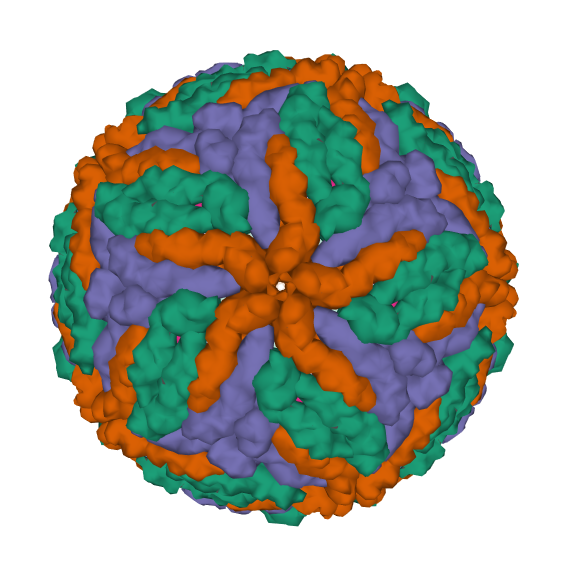
\includegraphics[width=4cm]{../figs/6CO8_assembly.png}
%    \end{minipage}
%
%\begin{tcolorbox}
%    Use Galerkin BEM code Bempp-cl accelerated with fast particle interactions through Exafmm
%\end{tcolorbox}
%
%Outline of rest of talk:
%\begin{itemize}
%    \item A short introduction to Bempp-cl and Exafmm
%    \item Black-box coupling strategies for Galerkin BEM
%    \item Practical issues and ongoing work
%\end{itemize}
%
%\end{frame}
%
%\begin{frame}
%    \frametitle{Bempp-cl}
%    \begin{itemize}
%        \item Successor of the Bempp boundary element library.
%        \item Fully developed using Python with fast OpenCL kernels for computational routines.
%        \item Galerkin discretisation of operators for Laplace, Helmholtz, and Maxwell problems.
%        \item Compute kernels can be run on CPU or offloaded to GPU.
%        \item Core routines optimised for fast dense assembly of opertors.
%        \item Library provides coupling interfaces to Exafmm, can be easily adapted to other
%            fast particle summation libraries.
%    \end{itemize}
%\end{frame}
%
%\begin{frame}
%    \frametitle{Characteristics of Bempp-cl}
%    \vspace{-.1cm}
%    \begin{center}
%        \begin{tabular}{cc}
%            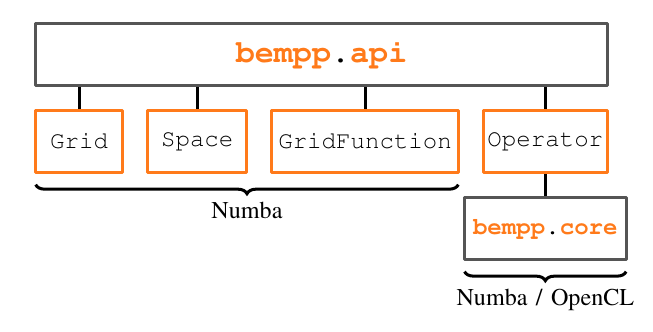
\includegraphics[width=5cm]{../figs/bempp_cl_overview.png} & 
%            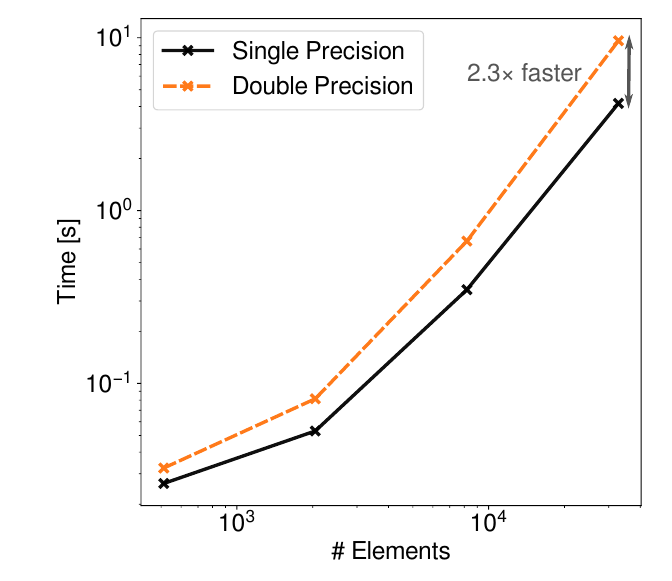
\includegraphics[width=5cm]{../figs/bempp_single_vs_double.png} \\
%            \begin{minipage}{5cm}
%                \vspace{-4cm}
%                \begin{itemize}
%                    \item Top: Structure of Bempp-cl
%                    \item Top-Right: AVX acceleration in Bempp-cl
%                    \item Bottom-Right: Offloading of a domain potential operator
%                \end{itemize}
%            \end{minipage}&
%            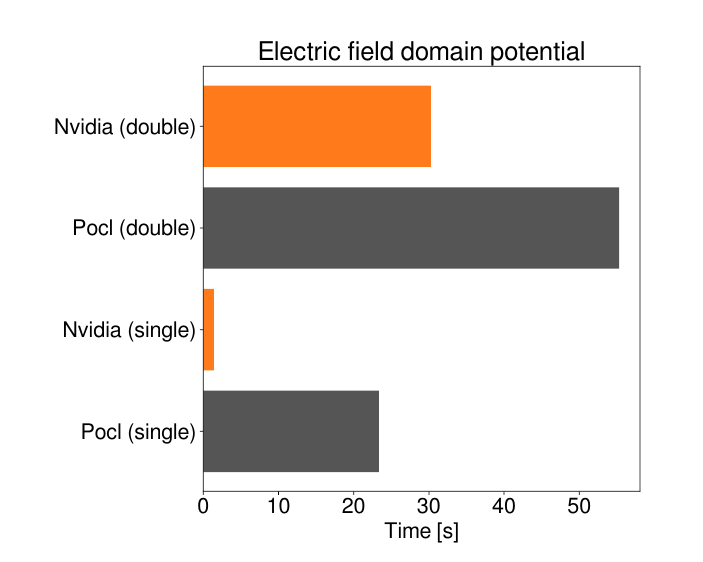
\includegraphics[width=5cm]{../figs/gpu_offloading.png} 
%        \end{tabular}
%    \end{center}
%\end{frame}
%
%\begin{frame}
%    \frametitle{Exafmm-t: High-Performance KIFMM}
%    \vspace{-.1cm}
%    \begin{center}
%        \begin{tabular}{cc}
%            \begin{minipage}{5cm}
%                \begin{itemize}
%                    \item Kernel-Independent FMM library.
%                    \item Written in C++, Provides Python Interface.
%                    \item Highly efficient at higher accuracies.
%                \end{itemize}
%            \end{minipage} &
%            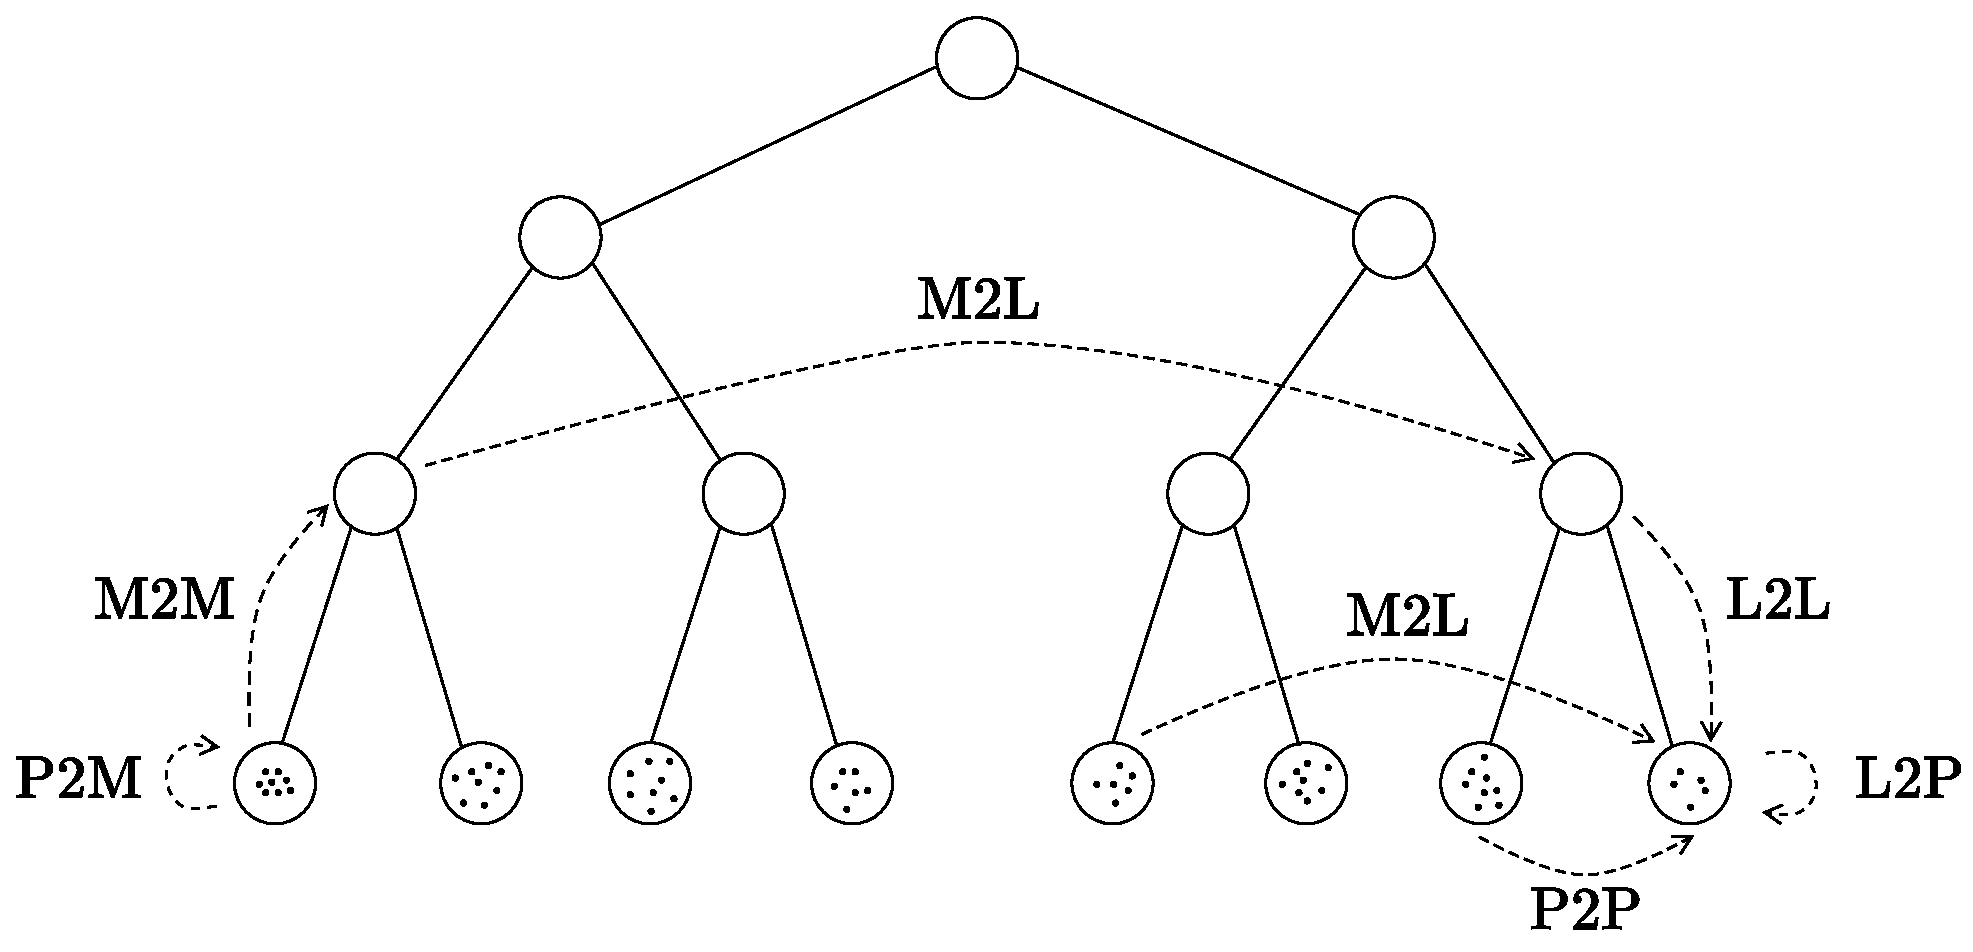
\includegraphics[width=5cm]{../figs/fmm_sketch.pdf} \\
%            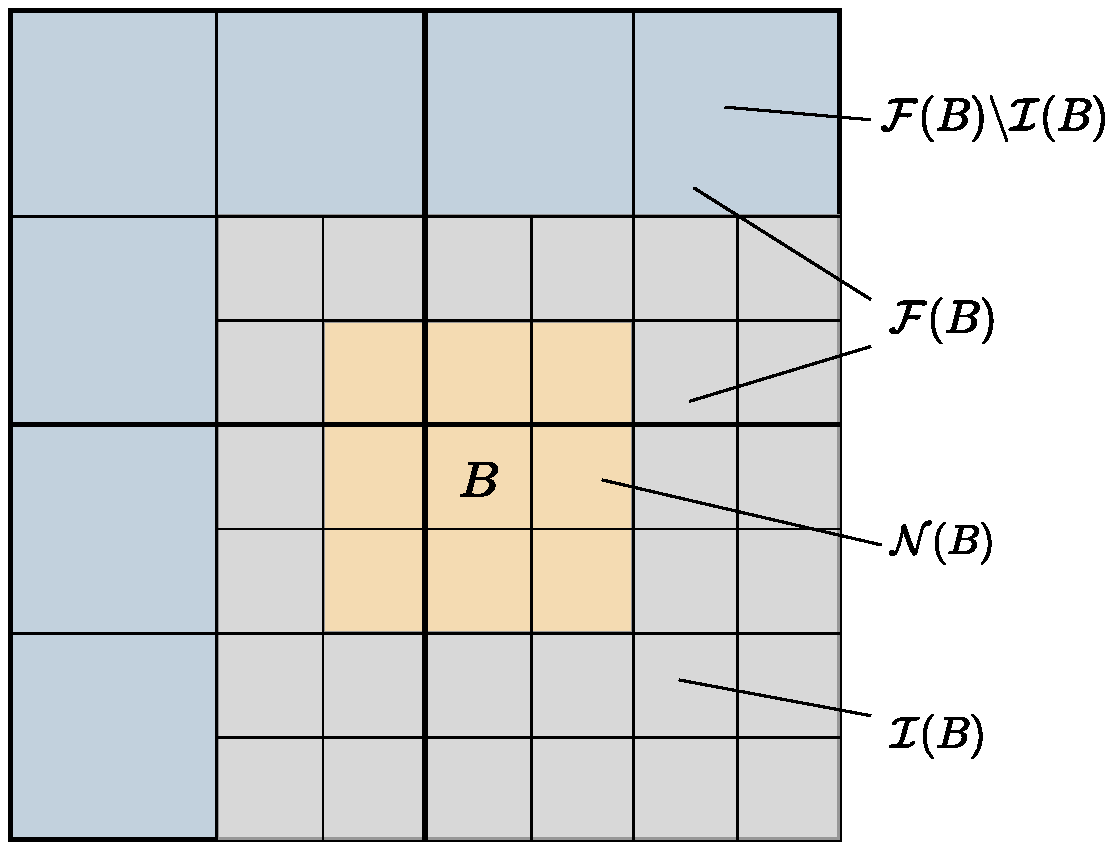
\includegraphics[width=4cm]{../figs/near_far_decomposition.pdf} &
%            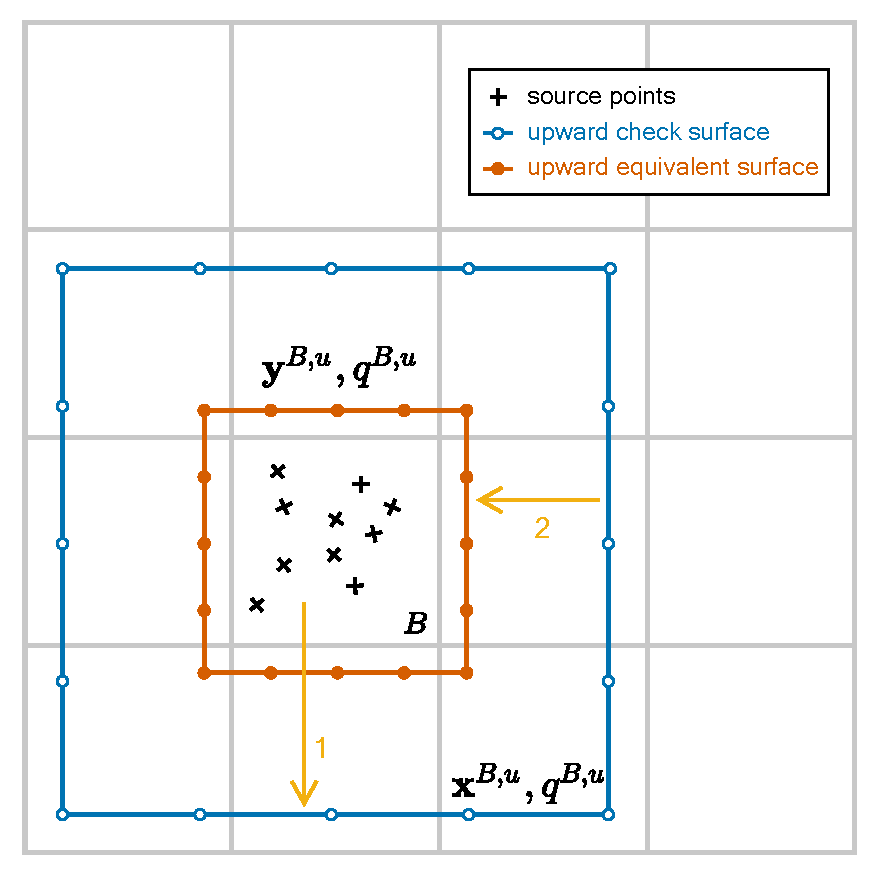
\includegraphics[width=4cm]{../figs/multipole_expansion.pdf}
%        \end{tabular}
%    \end{center}
%
%\end{frame}
%    
%\begin{frame}
%    \frametitle{Coupling Bempp-cl and Exafmm-t}
%
%Let $A$ be the matrix representation of a Galerkin discretised boundary integral operator.
%Let $x$ be any vector. Reformulate $Ax$ as
%
%$$
%Ax = P_{test}^T(G - C)P_{dom}x + Sx
%$$
%
%\begin{itemize}
%    \item $P_{test}$ and $P_{dom}$ highly sparse matrices that map function space coefficients to particle weights at quadrature points.    \item $G$ is black-box operator evaluating particle sums over weights across all quadrature points across all elements.
%    \item $C$ is sparse matrix that contains the particle interactions between neighboring triangles.
%    \item $S$ is sparse matrix containing all singular Galerkin integrals in adjacent elements.
%\end{itemize}
%
%\end{frame}
%
%\begin{frame}
%    \frametitle{The correction matrix}
%
%    \begin{center}
%        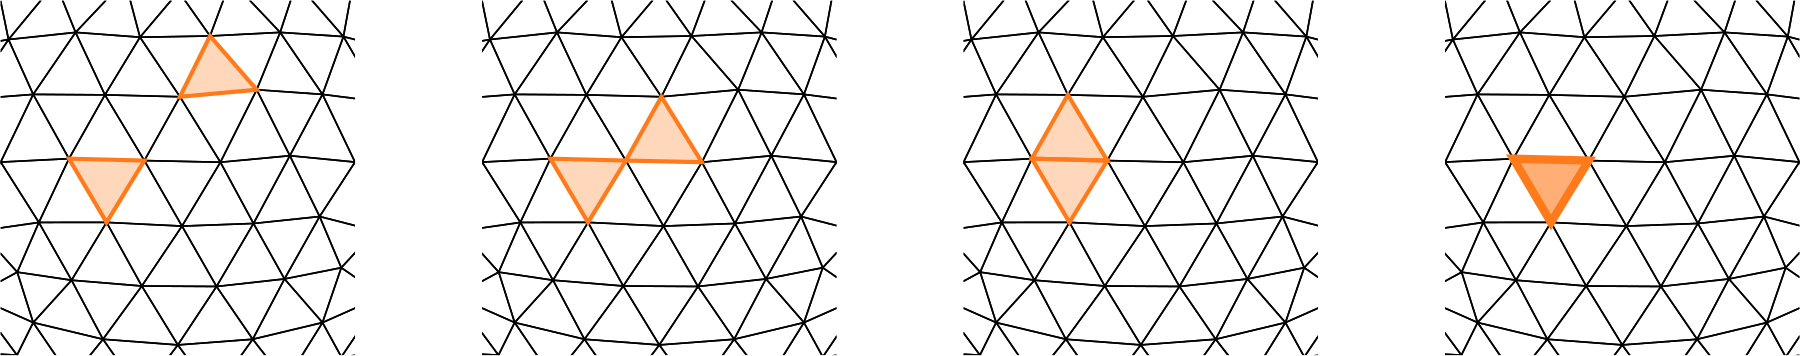
\includegraphics[width=10cm]{../figs/triangles.png}
%    \end{center}
%
%    Problem: Any FMM code also evaluates the near-field.
%    Near-field can contain adjacent triangles (singular quadrature rules), and
%    non-adjacent triangles (standard triangle Gauss rule).
%
%    \vspace{.5cm}
%
%    The sources and target points in the FMM are arising from the
%    non-singular quadrature rule.
%
%    \vspace{.5cm}
%
%    Solution: After FMM evaluation subtract out the regular quadrature rule
%    contribution from adjacent triangles and add in the correct singular quadrature
%    rule contribution.
%
%\end{frame}
%
%\begin{frame}
%    \frametitle{Number of FMM passes per Operator}
%
%    \begin{tabular}{c|c|c|c|c}
%        Operator & $V$ & $K$ & $K'$ & $W_Y$, $W_L$ \\
%        \hline
%        FMM Passes & 1 & 3 & 1 & 6, 3 
%    \end{tabular}
%
%    \vspace{.5cm}
%
%    Example: Double-Layer Potential Operator
%
%    \begin{align}
%        [K\phi](\mathbf{x}) &= \int_{\Gamma}
%        \partial_{\mathbf{n(\mathbf{y})}}g(\mathbf{x}, 
%        \mathbf{y})\phi(\mathbf{y})ds(\mathbf{y})\nonumber \\
%        &= -\sum_{j=1}^3\left[\nabla_{\mathbf{x}} 
%        g(\mathbf{x}, \mathbf{y})\right]_j\mathbf{n}_j(\mathbf{y})
%        \phi(\mathbf{y})ds(\mathbf{y})\nonumber
%\end{align}
%
%Require three FMM passes for the three different densities $\tilde{\phi}_j(\mathbf{y}):=\mathbf{n}_j(\mathbf{y})\phi(\mathbf{y})$, $j=1,\dots, 3$.
%
%\vspace{.5cm}
%
%The transmission operator for the exterior Poisson-Boltzmann formulation requires {\color{red} 19 FMM passes}.
%
%\end{frame}
%
%\begin{frame}
%    \frametitle{Poisson-Boltzmann for a sphere}
%
%    \begin{center}
%        \begin{tabular}{cc}
%            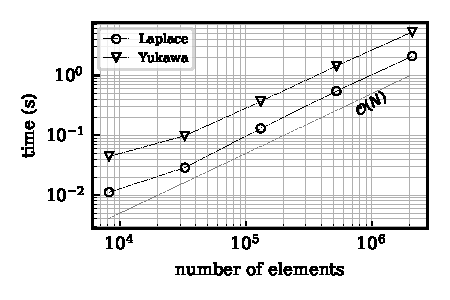
\includegraphics[width=5cm]{../figs/sphere_fmm.pdf} &
%            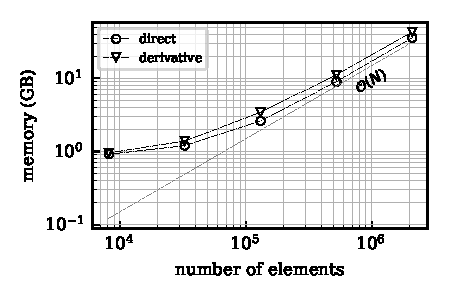
\includegraphics[width=5cm]{../figs/sphere_memory.pdf} \\
%            \begin{minipage}{5cm}
%                \vspace{-3.5cm}
%                \begin{itemize}
%                    \item FMM Expansion Order 5
%                    \item 6 regular quadrature points per element
%                    \item \textbf{Right} Blue: Laplace, 
%                        Yellow: Yukawa, Green: Singular Correction, Red: Other
%                \end{itemize} 
%            \end{minipage} &
%            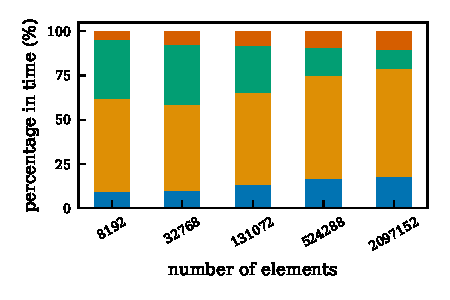
\includegraphics[width=5cm]{../figs/sphere_gmres_derivative.pdf}
%        \end{tabular}
%    \end{center}
%\end{frame}
%
%\begin{frame}
%    \frametitle{Results for Zika Virus}
%
%    \begin{center}
%        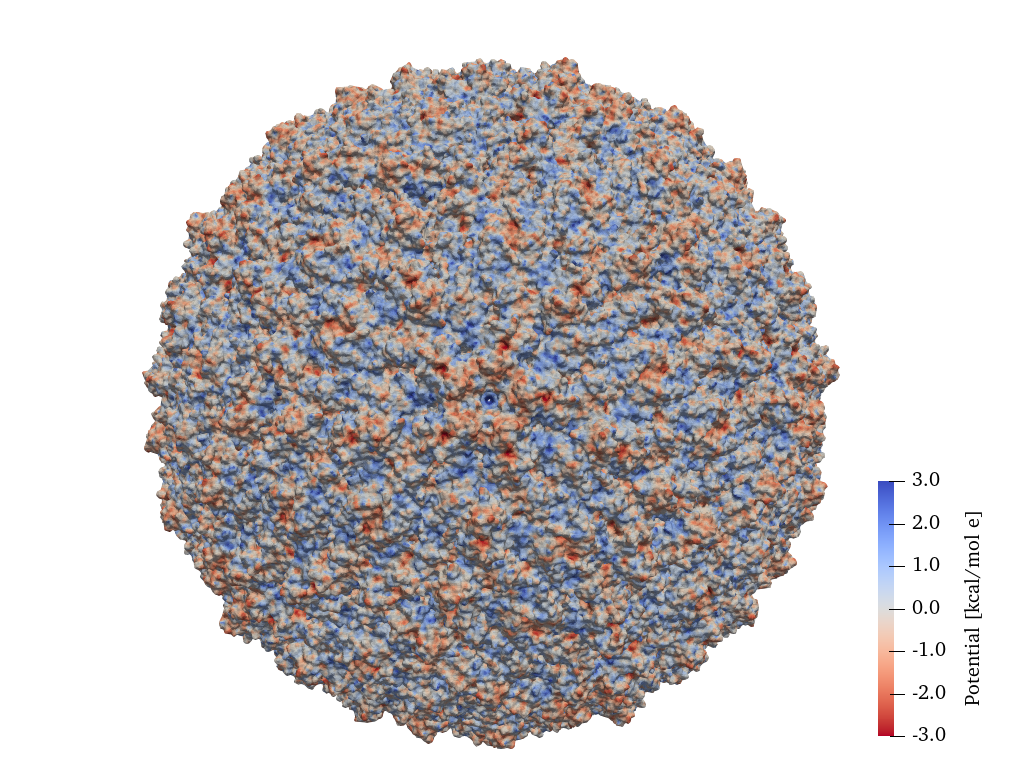
\includegraphics[width=8cm]{../figs/6CO8_potential.png}
%    \end{center}
%
%    40 Core Compute node. Total time: 139.5 minutes, GMRES time: 80 minutes, 18 GMRES iterations, Max RAM use: 43GB, $\Delta G_{solv} = -116254.9 kcal/mol$. Diagonal preconditioner through inverse of mass matrix with mass lumping.
%
%\end{frame}
%
%\begin{frame} 
%	\frametitle{A FEM/BEM formulation for inhomogeneities}
%	
%	Want to model the interior permittivity as variable. $\rightarrow$ Use FEM for interior/BEM for exterior domain.\\
%	(joint work with E. Burman, M. Bosy, C. Cooper)
%	
%	
%	\begin{center}
%  \textit{Find $ \phi_1 \in H^1(\Omega_1)$ and $\lambda_2 \in H^{-\frac{1}{2}}(\Gamma)$ such that for all $v \in H^1(\Omega_1)$ and $\zeta \in H^{-\frac{1}{2}}(\Gamma)$}
%\begin{equation}
%\nonumber
%\label{eq:standard_fem_bem}
% \left\{
% \begin{array}{rcl}
% \left(  \epsilon_1 \nabla \phi_1, \nabla v \right)_{\Omega_1}  - \left< \epsilon_1 \lambda_2, v \right>_\Gamma &=&   \left(  \sum_{k=1}^{N_q} q_k\delta(\mathbf{x},\mathbf{x}_k),  v \right)_{\Omega_1} \\[3mm]
%  \left< \left(\tfrac{1}{2} I - K_{Y}^{\Gamma}\right) \phi_1, \zeta \right>_\Gamma + \tfrac{\epsilon_1}{\epsilon_2} \left< V_{Y}^{\Gamma} \lambda_2, \zeta \right>_\Gamma &=&0.
%  \end{array}
%  \right.
%\end{equation}
%\end{center}
%
%Matrix form:
%
%\begin{align*}
%\begin{bmatrix}
%\epsilon_1 A &  - \epsilon_1 M^T \\
%\left(\tfrac12 I + K \right) &  \tfrac{\epsilon_1}{\epsilon_2} V
%\end{bmatrix}
%\begin{bmatrix}
%\vec{\phi}_1 \\
%\vec{\lambda}_2
%\end{bmatrix}
%=
%\begin{bmatrix}
%\vec{f} \\
%0
%\end{bmatrix}.
%\end{align*}
%
%Use FEniCS for interior problem, Bempp-CL for exterior problem.
%
%\end{frame}
%
%\begin{frame}
%\frametitle{FEM/BEM vs BEM/BEM for constant permittivity}
%
%\begin{figure}
%  \centering
%  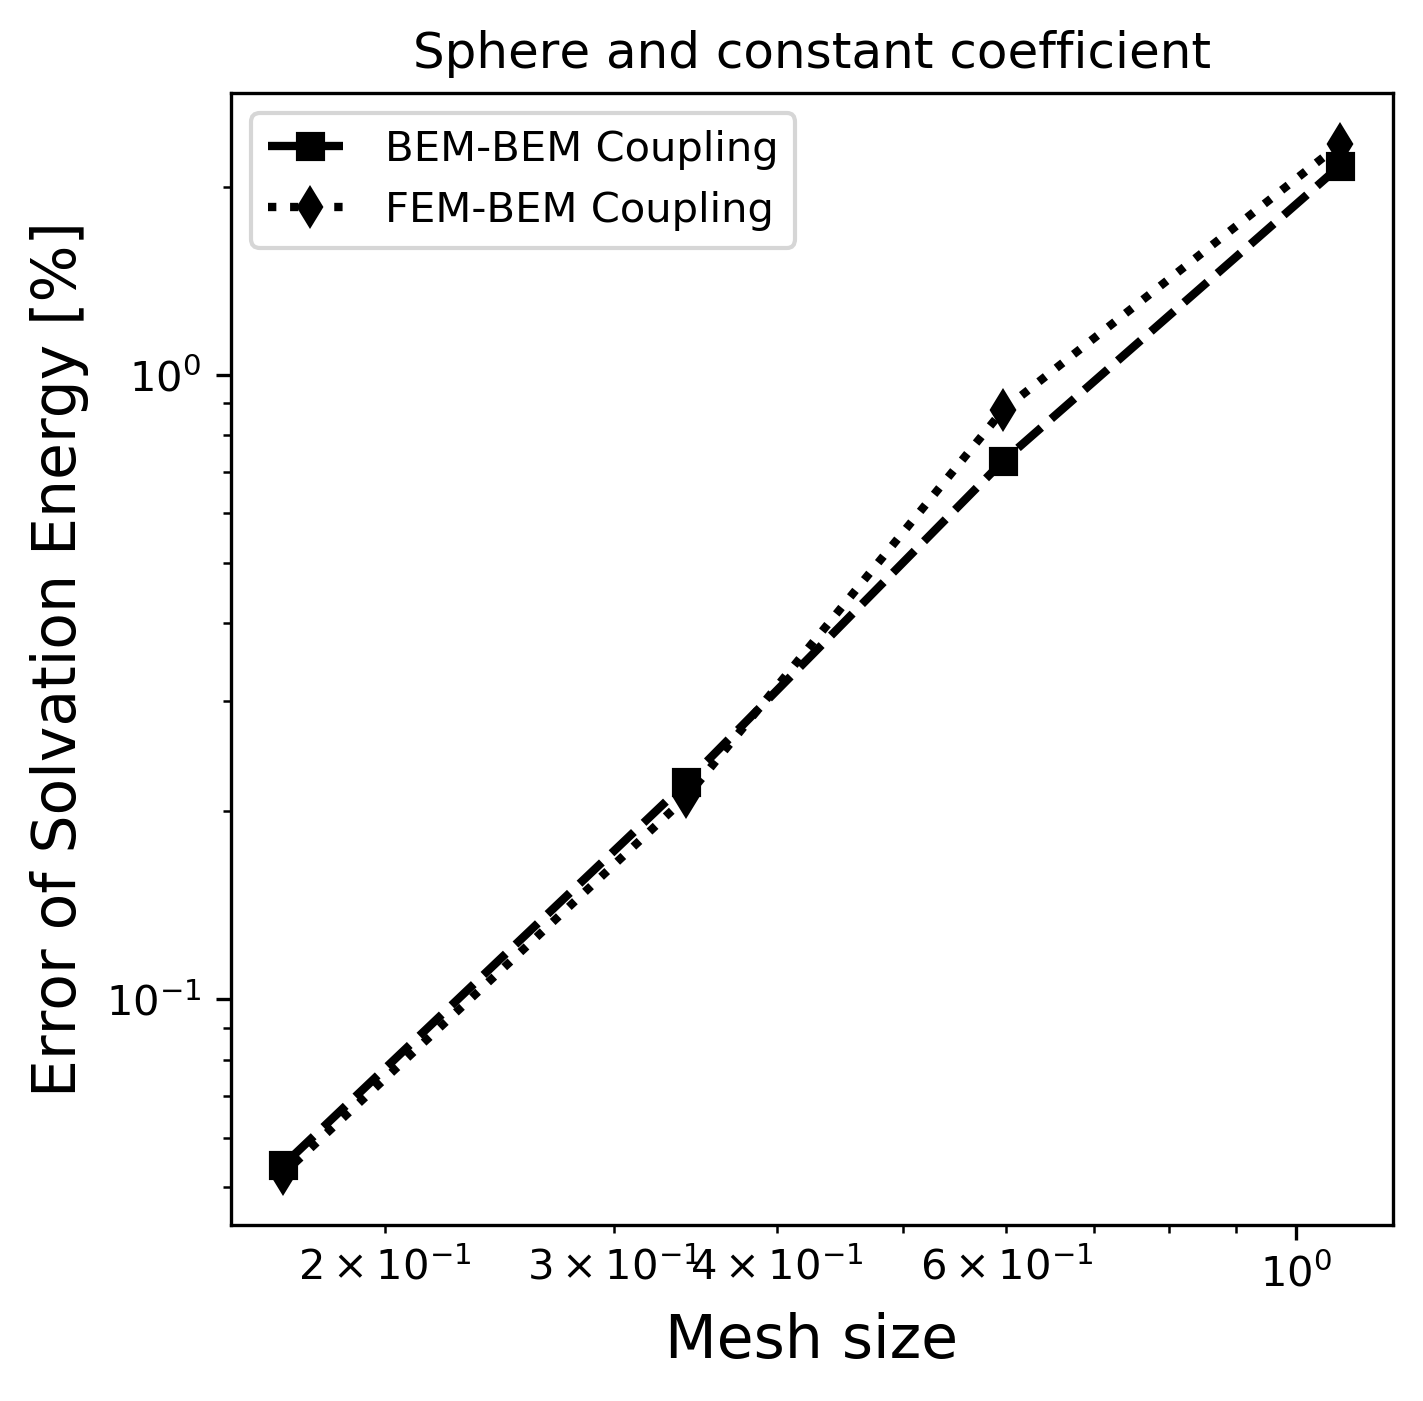
\includegraphics[width=0.6\linewidth]{../figs/Sphere_const_coeff_error.png}
%  \caption{Error for the Kirkwood sphere.}
%  \label{fig:error_sphere}
%\end{figure}
%\end{frame}
%
%\begin{frame}
%  \frametitle{Comparison with APBS - varying permittivity}
%\begin{table}
%\centering
%\begin{tabular}{c|c|c}
%&Mesh size & $\Delta G_{solv}$\\
%&\AA       &  kcal/mol \\
%\hline
%\multirow{4}{*}{APBS}& 0.52$\times$0.52$\times$0.52 & -32.4652\\
%& 0.39$\times$0.39$\times$0.39 & -32.4042\\
%&0.26$\times$0.26$\times$0.26 & -32.3375\\
%&0.17$\times$0.17$\times$0.17 & -32.3413\\
%\hline
%&Mesh dens. & \\
%&vert/\AA$^2$ & \\
%\hline
%%\multirow{5}{*}{Standard FEM-BEM}& 2 & -36.239\\
%    & 2 & -35.688 \\
%FEM-BEM    & 4  & -33.304 \\
%coupling    & 8  & -32.634 \\
%    & 16 & -31.868 \\
%\hline
%%\multirow{5}{*}{Standard FEM-BEM}& 2 & -29.554\\
%%    & 2 & -34.670\\
%%Hybrid    & 4  & -33.603 \\
%%FEM-BEM    & 8  & -32.822 \\
%%    & 16 & -32.072 \\
%%\hline
%\end{tabular}
%\caption{Solvation energy of arginine with a Gaussian-like permittivity, computed using the FEM-BEM approach and APBS. The mesh density for FEM-BEM corresponds to the vertex density of the surface mesh used to generate the volumetric mesh}
%\label{table:arg_variable}
%\end{table}
%\end{frame}
%
%
%\begin{frame}
%    \frametitle{A Rust based scalable fast solver framework}
%
%    \vspace{.2cm}
%    Goal: Create a fast solver framework for fast parallel forward evaluation and
%    approximate inversion of integral operators (\url{https://github.com/rusty-fast-solvers/roadmap})
%
%    \vspace{\baselineskip} 
%
%    {\color{blue} All component libraries developed in Rust with Rayon (multithreading)
%    and MPI (across nodes) for parallelization.}
%    \vspace{\baselineskip}
%
%    Development Status:
%    \begin{itemize}
%    \item {\color{blue} rusty-green-kernel} AVX accelerated direct evaluation
%        of Laplace, Helmholtz Green's functions. {\color{green} released}.
%    \item {\color{blue} rusty-tree} Serial and parallel Octree implementations.
%        Serial tree implemented. 
%        Parallel tree early stages. {\color{yellow} close to release}.
%    \item {\color{blue} rusty-compression} Fast randomized compression routines
%        for approximate low-rank matrices. {\color{green} released.}
%    \item {\color{blue} rusty-translation} Implementation of M2M, 
%        M2L, L2L, P2M, L2P operators
%        based on numerical field compressions (KIFMM, etc.)
%        {\color{yellow} early development}
%    \item {\color{blue} rusty-fmm} Serial and parallel FMM loops 
%        {\color{red} In planning}
%    \item {\color{blue} rusty-inverse} Evaluation of approximate inverses 
%        {\color{red} Not yet started}
%    \end{itemize}
%
%\end{frame}
%
%\begin{frame}
%    \frametitle{Summary}
%
%    \begin{itemize}
%        \item Generic, practically usuable and efficient black-box coupling of Galerkin
%            BEM and Exafmm.
%        \item All computational results shown today steered through interactive Jupyter
%            notebooks.
%        \item Python glue language between the codes. High productivity through Jupyter
%            interface.
%        \item For links to paper, reproducible data and codes see\\
%            \url{https://github.com/barbagroup/bempp_exafmm_paper}
%        \item Ongoing development of exascale ready software for EPSRC's new ARCHER2 system (AMD EPYC CPU Cluster)
%        \item Goal: Large-scale coupled Finite element/Boundary element models
%    \end{itemize}
%
%
%\end{frame}
%
%\begin{frame}
%    \frametitle{Papers}
%
%{
%    \small
%
%\begin{itemize}
%    \item T. Wang, C. Cooper, T. Betcke, L. Barba, \textit{High-productivity, 
%        high-performance workflow for virus-scale electrostatic simulations with 
%    Bempp-Exafmm}, arXiv preprint arXiv:2103.01048 (2021), 
%    \url{https://github.com/barbagroup/bempp_exafmm_paper}
%    \item T. Betcke, M. W. Scroggs, \textit{Bempp-cl: A fast Python based 
%        just-in-time compiling boundary element library}, 
%        Journal of Open Source Software, 6(59), 2879 (2021), 
%            \url{https://doi.org/10.21105/joss.02879}
%    \item T. Betcke, M. W. Scroggs, \textit{Designing a high-performance boundary 
%        element library with OpenCL and Numba}, 
%        Computing in Science \& Engineering 23, pp. 18--28 (2021) 
%        \url{https://doi.org/10.1109/MCSE.2021.3085420} 
%    \item T. Wang, R. Yokota, L. Barba, \textit{ExaFMM: a high-performance 
%            fast multipole method library with C++ and Python interfaces.}
%        Journal of Open Source Software, 6(61), 3145 (2021),
%        \url{https://doi.org/10.21105/joss.03145}
%    \end{itemize}
%
%}
%
%
%    \vspace{1cm}
%
%
%\end{frame}

\end{document}

